\chapter{Святой Кюрила}

Как его только не называли в летописях, монастырь сей. И святой Кюрила, Курило, и Кирилловский – суть не меняется. Познакомимся с монастырем и церковью, давшими имя высотам, а заодно со зловещими ярами по обеим сторонам горы, на которой стоит эта церковь.

От Смородинского спуска недалече. Я придерживаюсь положения, что упомянутые в сказаниях несколько пещер, где обитал Змей – это пещеры именно на Смородинском спуске. И что тамошняя спиралевидная пещера, описанная Антоновичем, она же главная героиня фильма «Логово Змия» – и есть упоминаемая в источниках Кирилловская или Змиева пещера.

Однако не всё так четко и ясно.

На привязку Змея к Смородинским пещерам указывает неясная штука – людская молва, изустное предание. Некие люди живут, помнят что-то, передают словами другим людям, а те далее, с течением времени. Так в народе сохраняется память. Быть может, несколько веков назад ребенок спросил у деда – а что это за пещера? Тот вспомнил – здесь жил Змей. Ребенок вырос, состарился, сам стал дедом, и уже в ответ своему внуку поведал ту же историю. Но если внук задал вопрос о другой пещере, близлежащей, а дед решил, что речь идет об известной ему, деду, пещере? Так молва способна перенести название с одной пещеры на другую, исказить предание.

И не грех обозреть окрестности, чтобы выяснить, какие еще тут существуют пещеры и подходят ли они под название Кирилловской. Именно Кирилловской, остальное нас не касается, потому что Кирилловская пещера однозначно связана с легендами со Змеем. Кирилловская пещера точно является Змиевой пещерой. Но является ли спиралевидная пещера на Смородинском спуске – Кирилловской пещерой? На этот вопрос нельзя ответить положительно с полной уверенностью, хотя по совокупности доводов можно так считать.

Рассмотрим вначале упрощенную карту, которая поможет в дальнейшем рассказе.

\begin{center}
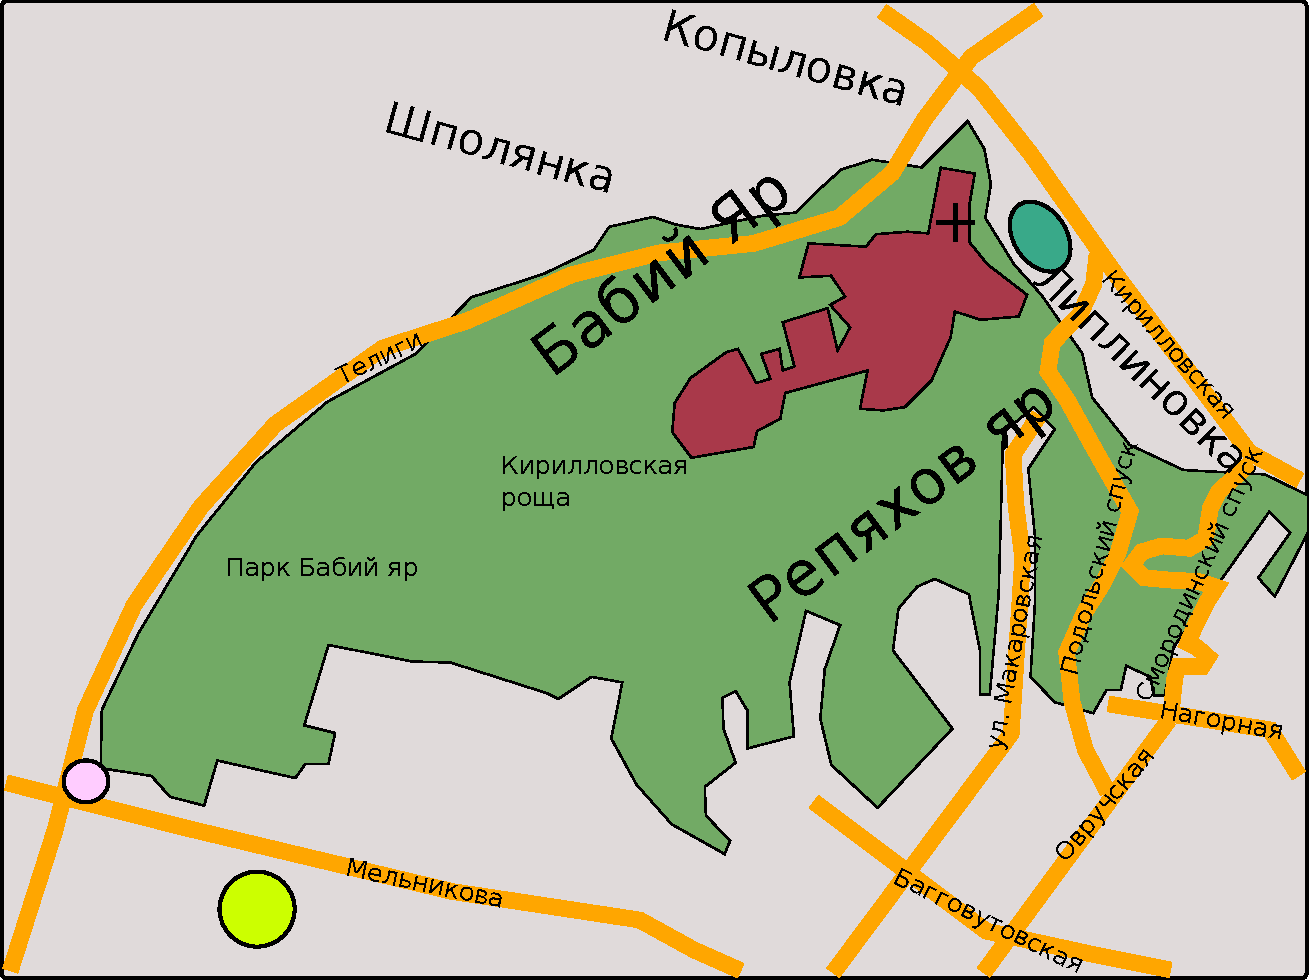
\includegraphics[width=\linewidth]{chast-zmiy/kurilo/kyr-okr.pdf}
\end{center}

Многие улицы я выпустил, лень было рисовать. Мне важно просто отметить взаимное расположение урочищ.

Крестом обозначена Кирилловская церковь. 

Зеленая область – парки, рощи, просто заросли.

Вишневого цвета область – территория психбольницы имени Павлова, бывший Кирилловский монастырь.

Улица Макаровская вообще-то делится на Пугачева и Макаровскую. Раньше границы Макаровской ездили туда-сюда, а северный отрезок нынешней Макаровской назывался улицей Мстиславской, которая иногда заменяла всю Макаровскую. Всё это неважно для предмета нашего разговора.

Салатовый кружок – телебашня.

Розовый кружок – станция метро «Дорогожичи».

Овал цвета морской волны – стадион «Спартак».

Теперь начнем повсюду бродить.

Под горой с церковью сейчас находится стадион «Спа\-ртак». У него старая еще, середины прошлого века, кованая, будто из скрепленных копий, ограда с буквами «С».

\begin{center}
\includegraphics[width=\linewidth]{chast-zmiy/kurilo/\myimgprefix IMG_2674.JPG}

\textit{Снимок 2013 года.}
\end{center}

13 марта 1961 года она была залита по самые наконечники пульпой. Годами, Петровские кирпичные заводы на Сырце\footnote{Сохранившийся от них карьер, ставший озером, находится по координатам 50°29'10.85"N 30°26'48.17"E. Это в двухста с лишком метров к югу от восьмидесятых номеров по улице Сырецкой.} гнали по трубам непригодную к производству породу, смешанную с водой, в Бабий яр, находящийся к северу за горой. Дамбу яра прорвало и отходы хлынули вниз. Грязь обрушилась на Куренёвку и погребла под собой сотни, если не тысячи людей. Об этом написано несколько книг и множество статей, это отдельный разговор, как и сам Бабий яр.

Гору с Кирилловской церковью издревле сторожили два длинных и глубоких яра – Бабий с севера и Репяхов с юга. Бабий яр известен в истории по учиненным гитлеровцами расстрелам в 1941 году и по Куренёвской трагедии 61-го. Пожалуй, трудно сыскать в мире место с более мрачной историей.

Сейчас некоторые пишут – мол, никаких расстрелов в Бабьем яру не было. Может и войны не было?

Осенью 1941 года в яру начались расстрелы – и первыми были убиты 752 пациента Павловки, психиатрической больницы на территории бывшего Кирилловского монастыря. Спустя два дня, 27 сентября, немцы «пригласили» в Бабий Яр евреев.

С ним связана беда и моих предков по материнской линии, хотя и не евреев.

Прадед и прабабушка, Федор Максимович и Марфа Семеновна Бородины в 1930-х перебрались в Киев из села Непхаево, что в Белгородской области. 

Сорваться с родных мест, где дети боярские (было такое сословие, оно же однодворцы) Бородины и Черняевы жили по крайней мере с 17 века, вынудили обстоятельства. Федор Максимович был среди братьев старшим, служил в колхозе конюхом. А брат его Охрим работал начальником железнодорожной станции в Самаре. И прислал большаку письмо – мол, растратил казенные деньги, что делать?

Федор Максимович продал дом, корову Зорьку, лошадь, и поехал со всей семьей – женой и дочкой Таней (моей бабушкой) в Самару. Там, отдав Охриму большую часть денег, Бородины купили себе домик «в центре города», однако не смогли там жить, потому что местные говорили на непонятном языке, были чужими.

Бородины вернулись в Непхаево, где над ними смеялись – дескать, ездили в погоне за длинным рублем! Бородины ведь скрыли охримову растрату. 
 
Федор Максимович подался на заработки (он был еще и столяром) в Харьков, а накопив денег и получив какой-то посул работы в Киеве, отправился с семьей сюда, где поселился в коммунальной квартире в подвальном помещении флигеля усадьбы Беляшевских, на Чкалова 43\footnote{В адресных книгах 1882 года по адресу Мало-Владимирская, 41 живет «священник Беляшевский», в 1899 году дом имеет номер 43, а живет там Стемпниовский А. М., и по крайней мере в 1906-1914 годах – «Стемпниовская Ольга Як.».}, квартира 28. Сейчас этот дом носит адрес Гончара, 43-В.

Федор Максимович устроился работать продавцом в продуктовом магазине «на Золотоворотской улице», а потом столяром в «военную часть» неподалеку. Марфа же работала уборщицей у военных в доме около Золотых ворот, а потом уборщицей в НКВД и рассказывала, как нквдшники рассовывали себе по карманам лежащие на столах конфискованные украшения, а она подбирала упавшие и клала обратно на стол.

От военной части Бородины получили комнату в коммунальной квартире в семиэтажке напротив пожарного депо на Короленко (Владимирской), 13. Позже, после взрыва здания немцами, переселились на второй этаж самого депо.

Тут я несколько путаюсь, потому что бабушка говорила и про частичный взрыв дома на Чкалова, и что потом его восстанавливали после войны. И в какой военной части работал прадед, тоже непонятно – возможно на улице Ярославов вал.

На пригорке над домом на Чкалова\footnote{Улица перпендикулярна к Ярославову валу, спускается от него вниз.} в самом деле была «военная часть», и от нее сохранился довоенный еще бункер, ниже дома Сикорских (Ярославов вал, 15-Б). Вообще этот бункер во время войны относился к штабу и командному пункту Киевского корпуса ПВО (7-й корпус ПВО). До войны, командный пункт в бункере (Ярославов вал, 15-А) был в распоряжении 3-й дивизии ПВО, по крайней мере с 1938 года.

Над бункером, выше по горе – уцелевший дом Сикорских. Он стоит во дворе выходящего на Ярославов вал пятиэтажного серого здания под номером 15, известного как бывшая военная гостиница «Красная звезда». Она построена на месте одноэтажного другого дома Сикорских. В обоих и старых зданиях, и позже в нововыстроенном размещался штаб ПВО. Командный пункт около бункера был в ведении ПВО до 1968 года.

На горке между трехэтажным домом Сикорских и флигелем Беляшевских еще в советское время построили также белопанельный дом для высшего командного состава, но там жили и партийцы да ученые, в том числе академик Глушков. Бункер же в 70-е переоборудовали под убежище гражданской обороны.

По словам бабушки Тани, немцы при отступлении «за Днепр» выгоняли всех из близлежащих домов, и дом где Бородины жили частично взорвали. О каком доме идет речь – на Чкалова или Короленко – я не понимаю. Изгнанная из дому, прабабушка Марфа с маленьким сыном Сашей перебралась в деревню Кожанку Киевской области, под Фастовом. 

Этому предшествовала гибель Федора, после которой Марфа и Саша пряталась сначала в лесах под Киевом, комнату же занял дворник. Здесь я свожу воедино данные из рассказов бабушки разных лет, поэтому очень сложно. Бабушку в описываемое время, еще до смерти ее отца, угнали в Германию. А прабабушка после освобождения Киева, вернулась в город и жила где-то на Большой Житомирской.

Где бы ни жили Бородины во время войны – на Короленко ли, на Чкалова ли, у них были соседи – еврейская семья, супруги, с дочкой примерно пяти лет, по имени Майя. Отец Майи еще до войны был военным и с нападением фашистов ушел на фронт, а жена его с дочерью остались в Киеве.

Мать Майи отправилась в Бабий яр, а Майю Бородины спрятали сначала у себя, а потом Федор Максимович куда-то ее переправил в безопасное место, к родственникам девочки или к знакомым, непонятно.

После этого другие соседи «заложили» Бородиных (за такую услугу немцы платили), в подвал пришли полицаи и отвели Федора Максимовича в гестапо, где фрицы его избили, и как бабушке потом рассказывали – ее отец умер от побоев уже в Октябрьской, ныне Александровской больнице и похоронен там в братской могиле, которую я не могу найти.

В конце семидесятых, при строительстве на территории больницы, во время земляных работ находили черепа.

Несколько раньше Бородиным удалось спасти военного врача, Николая Филипповича (Пилиповича) Шило из села Александровки Бобровицкого района, Черниговской области. При отступлении советских войск судьба забросила его в Киев к двоюродному брату, того не оказалось дома, но приютили Бородины, лечили и кормили, пока в городе не стало совсем опасно. 

Николай начал пешком пробиваться домой, вместе с моей бабушкой Таней, которую родители хотели отправить подальше от города. Три дня пешком до станции Кобыжчи. Позже, как только бабушка вернулась в Киев – потянуло проведать – её угнали на работы в Германию. И Шило, узнав об этом, рвал на себе волосы и говорил: «Зачем я ее отпустил в Киев?».

А попасть в Германию было очень просто – идешь себе к Сенному рынку, вдруг облава, оцепление, тащат в немецкую комендатуру на Артёма, 24. И наутро, как есть, без вещей, везут на вокзал и грузят в полувагоны для скота, без крыши и дверей. Пересадка в Дрездене. Потом – «биржа труда», являются местные бюргеры на велосипедах, выбирают себе в рабы славян.

В Бабьем яру расстреливали не только евреев – жертвами пали военнопленные, цыгане, коммунисты, подпольщики. В 1943 году, когда наши освободили Киев, побывал там и корреспондент «Правды» Борис Полевой. Потом он вспоминал:

\begin{quotation}
Мы вошли в Киев с первыми советскими частями.  Город еще пылал. Но всем нам корреспондентам, не терпелось побывать в Бабьем Яру. О нем мы слыхали в эти годы предостаточно, но нужно было увидеть все самим. Сейчас уже не помню фамилию той женщины, которая взялась нас туда проводить. Помню только, кажется, что она была учительницей и пережила оккупацию. Мы приехали на Бабий Яр и обмерли. Громадные глубоченные рвы. Накануне бомбили город, и одна из бомб попала в откос яра. Взрывом откололо внизу кусок склона. И мы увидели непостижимое: как геологическое залегание смерти – между слоями земли спрессованный монолит человеческих останков. Даже в самом страшном сне такое не привидится... Не верилось, что все это может быть. Страшно... Очень страшно даже вспоминать об этом... Более страшного я не видел за всю войну. Потом были Освенцим, Дахау, Бухенвальд, десятки других мест массового уничтожения людей. Но самое страшное, уму непостижимое было там, в Бабьем Яру.
\end{quotation}

На снимках Johannes Hahle, фотографа 637-го немецкого отряда пропаганды 6-й армии Вермахта –  Бабий яр в 1941 году. Пленные советские граждане закапывают тела и вещи убитых.

\begin{center}
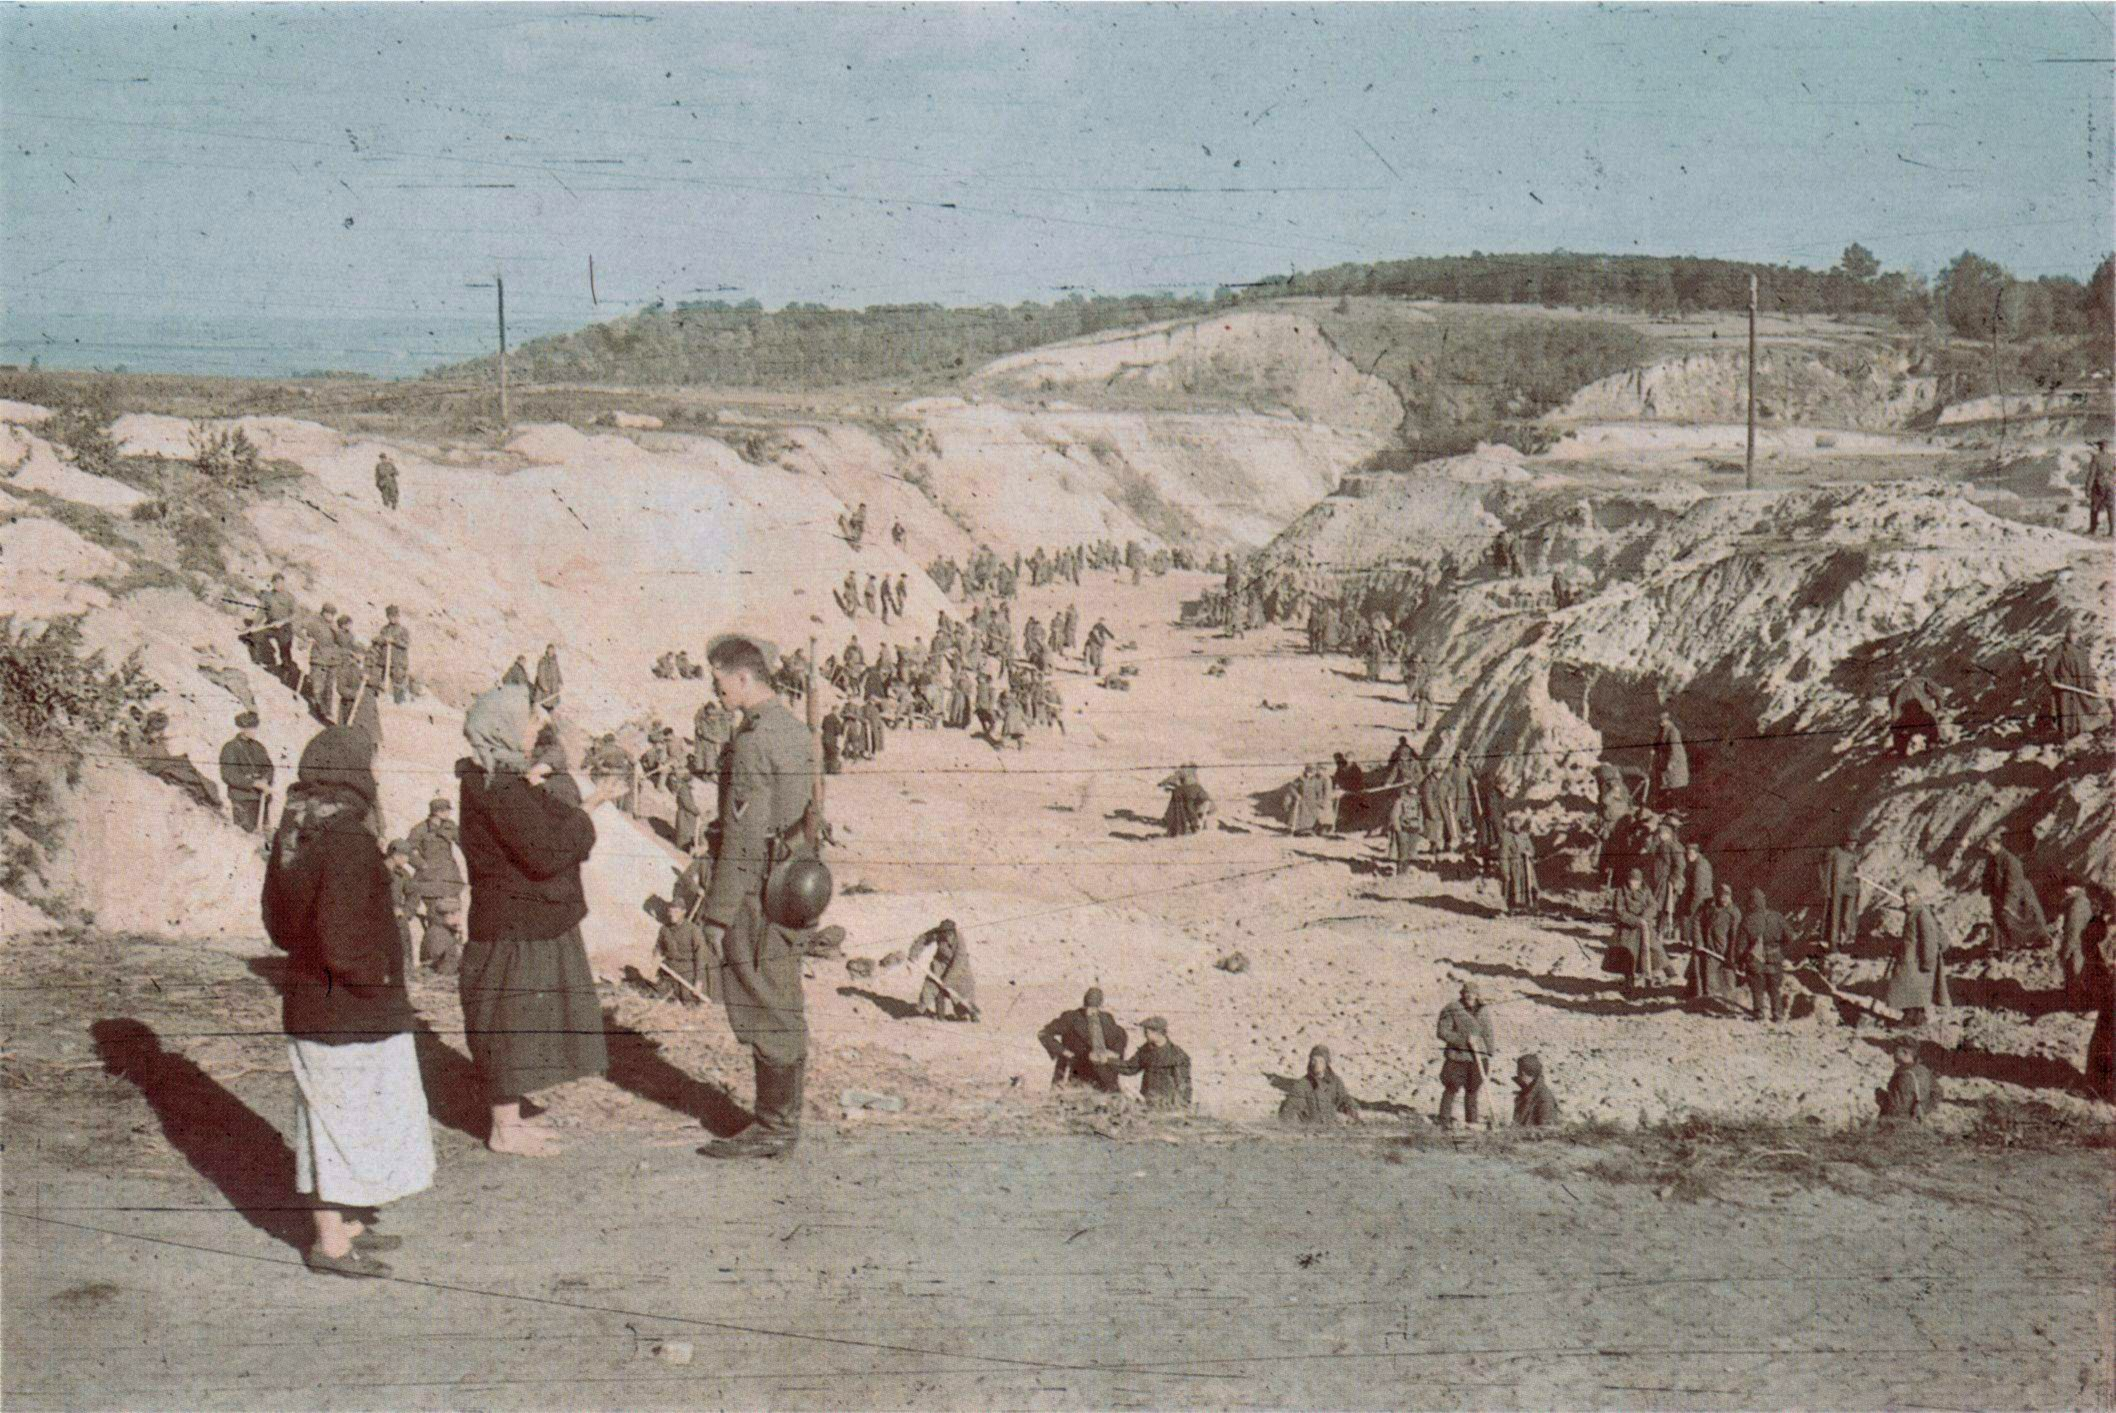
\includegraphics[width=\linewidth]{chast-zmiy/kurilo/byar-01.jpg}
\end{center}

\begin{center}
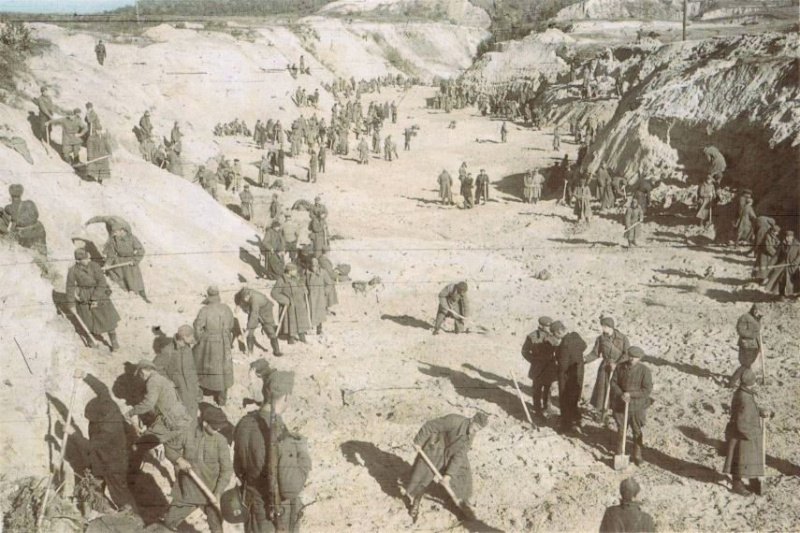
\includegraphics[width=\linewidth]{chast-zmiy/kurilo/byar-02.jpg}
\end{center}

До войны Бабий яр считался одним из наибольших киевских оврагов. Глубина его достигала 50 метров, а длина приближалась к трем километрам. По дну протекал Кирилловский ручей, ныне перехваченный бетонными желобами, уходящими в коллектор.

О каких-либо поселениях на берегах яра мне неизвестно, хотя соседний Репяхов яр был относительно обжит на стыке 19-20 веков. Происхождение названия Бабий яр неясно. В жалованных грамотах начала 15 века\cite{sofiasobor01} доминиканскому монастырю упомянуто на Нижнем Сырце урочище Хлопач или Пашня, прежде принадлежащее некой женщине Бисовой Бабе.

Причем в ранних грамотах описание, как мне кажется, размыто – его можно трактовать и вышеприведенным, и несколько иначе, что речь шла о двух урочищах – Хлопаче (принадлежавшем просто некой женщине) и Бисовой Бабе. В грамотах после 1411 года введено уточнение, задающее однозначную трактовку. А вот в «Записках о Киевском доминиканском монастыре» за 1634-1664 годы, генеральный проповедник в киевском доминиканском конвенте Петр Развидовский, описывая монастырские владения, упоминает отдельное урочище «Бесова баба»\cite{sbornikmat}:

%В грамоте князя Олелька Владимировича доминиканскому монастырю, 1411 года, говорится о правах на пошлины и перечисляются монастырские владения, жалованные Владимиром Ольгердовичем и Витовтом:

%\begin{quotation}
%Nos autem, his visis seu consideratis, dictam donationem vel eleemosynam patris Nostri iam dicti duximus confirmandam, praesentibusque confirmamus: velut theloneum, vulgo Poklodne, ut ex antiquo tenuerunt et recipiebant, villamque in ulteriori Syrecz sita, et allodium, dictum Chlopacz vel Paschnia, quae bona fuerunt cuiusdam foeminae, dictae Biesowa baba, cum omni jure, dominio omnibusque proventibus, quicunque in dictis bonis fuerunt vel fieri possint [...]
%\end{quotation}

%Строка «et allodium, dictum Chlopacz vel Paschnia, quae bona fuerunt cuiusdam foeminae, dictae Biesowa baba, cum omni jure» насколько я разбираю латынь, трактуется двояко. Первое – «Хлопач или Пашня, принадлежавшая некоторой женщине, называемой Бисова Баба, со всеми правами». Второе – «Хлопач или Пашня, принадлежавшая некоторой женщине, Бисова Баба, со всеми правами».

%Речь идет либо о Хлопаче (Пашне), что некогда была собственностью Бисовой Бабы, либо о двух отдельных урочищах – Хлопаче и Бисовой бабе.

%Praeterea villam na Zadnim Siercu cum praedio in terra dicta Chlopacz, quae bona quondam fuerunt cuispiam mulieris, dictae Bieszows Baba.

%, как пишут справочники без ссылки на источник, получило свое название от стоящего тут трактира, принадлежащего некой «бабе-шинкарке». И мол, она отдала свой земельный участок Доминиканскому монастырю, в 1401 году.

%Эти сведения сомнительны по самой уже дате. Если же их сместить на пару веков вперед, тоже не катит. В земельных польско-литовских документах не писали «баба-шинкарка», а указывали конкретные имена, к тому же неясно, зачем держать шинок в яру, где нет дороги и никто не живет.

\begin{quotation}
Там же на Сырце конвентских подданых десять.

Далее следуют грунты, названные Попковцы, где издавна некогда бывала деревушка до самой нивы, названная Плоцкая. [...]

Далее едучи от сей нивы в левой стороне грунты архимандричьи (печерские), а в правой наши, деревня Берковец; половина деревни Клашторной по самую часовню, которую мы построили, а другая половина – архимандричья. Их грунты идут на две мили к Белогородку, даже до Бесовой бабы, а наши грунты идут даже до Хлопача ко Гостомлю над Ирпенем.
\end{quotation}

Что, если в ранних грамотах напутано, и Бесова баба – таки урочище? Тогда, тождественны ли Бабий Яр и Бесова баба? Если да, то поразмыслим. Бабами издавна называли идолов – каменные бабы. А тут еще дополнительное указание – «Бесовая баба». Бесами после принятия христианства именовали поганских богов. Вдобавок, многие крупные монастыри Киева возникли на священных для язычников местах. Предположим, в Бабьем яру, точнее над ним, стоял некогда идол, баба. Не на месте ли Кирилловской церкви?

Александра Шандаренко в документальной книге про немецкую оккупацию Киева «Регистраторша ЗАГСа. Из дневника киевлянки», пишет: «Бабий Яр. Длинные, глубокие, извилистые яры, где когда-то на Ивана Купалу и на зеленый праздник Троицы женщины жали серпами высокую траву». Значит, в сороковых годах века двадцатого было еще памятно это поганское действо.

В 1944-м один из участков Бабьего яра передали во временное пользование карьероуправлению Горкомхоза для добычи глины. По пятилетнему плану 1946–1950 годов, в окрестностях Бабьего яра собирались сделать парк – что осуществили много позже. 

Трагически известная заливка отрогов яра пульпой с Петровских кирпичных заводов (по трубам от Сырецкой улицы) – итог сразу двух начинаний.

Заводам надо было сбрасывать куда-то пульпу\footnote{Пульпа вскрышных пород – при разработки глиняных карьеров в пойме Сырца производилась «вскрыша» – съем больших слоев грунта над полезной глиной. Съем выполнялся способом гидромеханизации – растворении в воде и отсоса земнасосом либо земснарядом. Жижа из воды и частиц грунта и называется пульпой.}, да и  в пятидесятых возникла необходимость проложить дорогу для соединения Куренёвки с верхним плато и замыкания кольца основных магистралей, и решили, что хорошо бы Бабий яр засыпать.

%Решение об этом приняли еще в 1950-м. За подписью начальника отдела планировки и застройки Киева М. Козлова вышло решение:

%\begin{quotation}
%Отдел планировки и застройки города не возражает против замыва отрогов Большого Яра, подходящих к территории вскрыши Сырецких заводов, на полную глубину. При проектировании учесть, что вдоль низа яра, находящегося на ул. Фрунзе, должен быть обеспечен в будущем выезд, с уклоном не более 4\%. В отношении возможности засыпки верховьев Бабьего Яра будет сообщено дополнительно.
%\end{quotation}

%В дальнейшем обсуждении проекта речь пошла о заливке всех трех крупных отрогов Бабьего яра. 

В 1961 году такое надругательство над природой и памятью дало о себе знать Куренёвской трагедией. А по засыпанным участкам яра стали проводить Новоокружную магистраль. Сейчас это улица Телиги от метро «Дорогожичи» и до Кирилловской. 

Вообще некоторые считают, что весь Бабий яр засыпан и от него почти ничего не осталось. Это не так. Основная его часть сохранилась в той или иной мере. Проще всего в этом убедиться на местности, шагая улицей Телиги вдоль холма с больницей Павлова и Кирилловской церковью.

Неподалеку остановки «Музей Кирилловская церковь» окажется, что по обеим сторонам улицы – заметные горбы. Это и есть берега низовий Бабьего яра, ранее бывшего здесь много глубже. Северный склон и ныне местами достаточно крут. Он прячется за чащей, куда бомжи нанесли толстый слой мусора. Гора обросла деревьями и уменьшились оползни.

Наибольшая область основного отрога яра уцелела и находится в современном парке Бабий яр, примерно напротив Февральского переулка и остановки «Больница имени Павлова». У остановки, направо от асфальтовой дороги, что идет к больнице, сворачивает тропинка. Она поднимается на громадную, с бетонным основанием плотину поперек яра. Она сравнительно новая, не та, которую прорвало.

Спускаемся по плитам. Ими же уложена дорога по дну яра. Громадные деревья подпирают левый, южный берег, неловко пытаясь скрыть могучую, древнюю его высоту. На гребень можно выбраться обходом, и встать вровень с кронами. Страшно!

Идем дальше. Постепенно начинает повышаться дно яра – не знаю, так ли было раньше. Всё здесь пронизано системой водоотвода. Она собирает ливневые потоки да многочисленные ручьи от родников. По бетонным желобам вода следует в общий коллектор. Ручьи на любой вкус и цвет – прозрачные, красно-бурые, обильные, полувысохшие. Вода движется, желоба соединяются. Остались и естественные русла.

Кое-где можно подобраться ко склону, есть лёссовые обрывы того масштаба, каков виден на фотографии Кирилловской стоянки, снятой Хвойкой. У подножия одной такой суглинной стены – болотце и ручей, вид совершенно первобытный.

Если пройти в направлении психиатрической больницы, будет длиться желоб с водой, и по правую руку склон, да еще один родник, сокровенный. В нем, студеном и чистом, плавает червь.

\begin{center}
\includegraphics[width=\linewidth]{chast-zmiy/kurilo/\myimgprefix byar-IMG_20140712_143446.jpg}

\textit{Улица Телиги, справа – остатки северного склона яра. 2014 год.}
\end{center}


\begin{center}
\includegraphics[width=0.96\linewidth]{chast-zmiy/kurilo/\myimgprefix byar-IMG_20140712_143940.jpg}

\textit{Вид с плотины. 2014 год.}
\end{center}

\begin{center}
\includegraphics[width=0.96\linewidth]{chast-zmiy/kurilo/\myimgprefix byar-IMG_20140712_144120.jpg}

\textit{Дорожка по яру. 2014 год.}
\end{center}

\begin{center}
\includegraphics[width=\linewidth]{chast-zmiy/kurilo/\myimgprefix byar-IMG_20140712_144453.jpg}

\textit{Часть системы водоотвода. 2014 год.}
\end{center}


\begin{center}
\includegraphics[width=\linewidth]{chast-zmiy/kurilo/\myimgprefix byar-IMG_20140712_144504.jpg}

\textit{Сплошной многометровый лёсс. 2014 год.}
\end{center}

\begin{center}
\includegraphics[width=0.95\linewidth]{chast-zmiy/kurilo/\myimgprefix byar-IMG_20140712_144545.jpg}

\textit{Источник под склоном. 2014 год.}
\end{center}

В 1960-х, в окрестностях, на улице Мельникова (бывшей Дорогожицкой) уничтожили кладбища – на месте Караимского и Старо-еврейского выстроили телецентр и спорткомплекс ДСО «Авангард», а на старой части Братского кладбища поставили телебашню. С краю отрога Репяхового яра остался кусочек Еврейского кладбища, и много надгробий сброшены в овраг под ним. Не знаю уж когда исчезло кладбище, которое было через яр напротив Кирилловской церкви, в прямоугольнике между улицами Захаровской, Петропавловской (бывший Петровский переулок) и Телиги.

В начале семидесятых на остатках верховий и середины Бабьего яра разбили парк, куда теперь обычно добираются через станцию метро «Дорогожичи». Двигаясь оттуда на северо-восток, мы попадаем в Кирилловскую рощу, предшествующую территории бывшего Кирилловского монастыря, а ныне психиатрической больницы имени Павлова, или Павловки. В этой роще, ранее – Кирилловском кладбище – встречаются могильные камни, здесь же у дороги стоит изуродованный склеп братьев Качковских, один из которых был известным в городе врачом. Тут покоились «доктор медицины Петр Эразмович Качковский и студент юрист Антон Эразмович Качковский». Покоились в прошлом, ибо тела давно исчезли, а подземные камеры наполнены мусором.

Добротно мощеная камнем дорога через чащу приводит нас к первым корпусам больницы. Южнее – недостроенное здание Института социальной и судебной психиатрии и наркологии, в народе Дурка. Тут всегда можно встретить неформалов, скалолазов и просто подозрительных типов. А севернее этой заброшки – огражденный не хуже концлагеря Городской центр судебно-психиатри\-ческой экспертизы. Его ворота имеют особенность, под ними огромный зазор.

Далее на восток, уже корпуса самой больницы и хозяйственные постройки – пищеблок, поликлиника, зал для проведения разных мероприятий. Многие стены разрисованы замечательными граффити. Домик с солнечной батареей, и рядом, на постаменте – покрытый серебрянкой бюст усатобородатого вивисектора академика Павлова. 

%Общество считает нормой одно, а ненормальным – другое, и носителей «ненормальности» стремится вернуть в лоно общепринятого движения мыслей, вроде – а давайте потратим столько-то миллиардов на вооружение, ведь убивать это самый простой и быстрый способ решения спора. Это норма. Чудака же, беседующего на улице с самим собой, называют безумцем, ставят ему диагноз и выписывают порошки. На-тко, лечись! Считай атомную бомбу нормой.

От былого монастыря, упраздненного задолго еще до революции 1917 года, осталось не так уж много – по большому счету сама Кирилловская церковь, да остатки стены середины 18 века, с башней-куполом. Стена принадлежит времени, когда архитектор Григорович-Барский выстроил тут несколько зданий. К более поздней, но все же дореволюционной старине относятся некоторые действующие корпуса больницы и одноэтажная бывшая прачечная, 1823 года, оформленная под дома бюргеров в баварских городках – ныне это корпус 10, морг, «Патанатомия». Она стоит неподалеку от церкви на север, рядом с лестницей, что спускается к улице Телиги. Прежний же старинный морг с часовней, постройки 1902 года, вероятно сооруженный на месте давней трапезной, ныне стал трапезным храмом Святителя Василия Великого.


Кирилловской церкви коснусь подробнее. Не будем забывать, что Хвойка обозначил на своей карте (смотрите главу про Кирилловскую стоянку) две пещеры – одну возле северо-западного угла церкви, другую – неподалеку, на склоне в сторону Кирилловской улицы.


\begin{center}
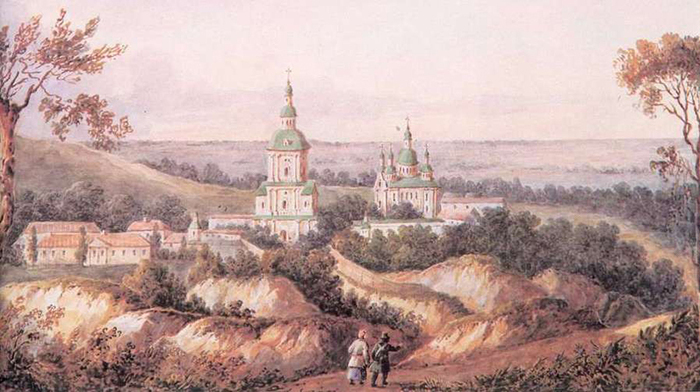
\includegraphics[width=\linewidth]{chast-zmiy/kurilo/Solncev_Kirilovskii_monastir_vozle_sela_Kyrenevka.jpg}

\textit{Федор Солнцев. Кирилловский монастырь возле села Куреневка. Акварель. 1843.}
\end{center}

\begin{center}
\includegraphics[width=0.60\linewidth]{chast-zmiy/kurilo/\myimgprefix kyr-cerk-IMG_20140712_142911.jpg}

\textit{Вход на территорию церкви платный. Плата не идет на пользу состоянию здания. 2014 год.}
\end{center}

\newpage
\vspace*{\fill}
\begin{center}
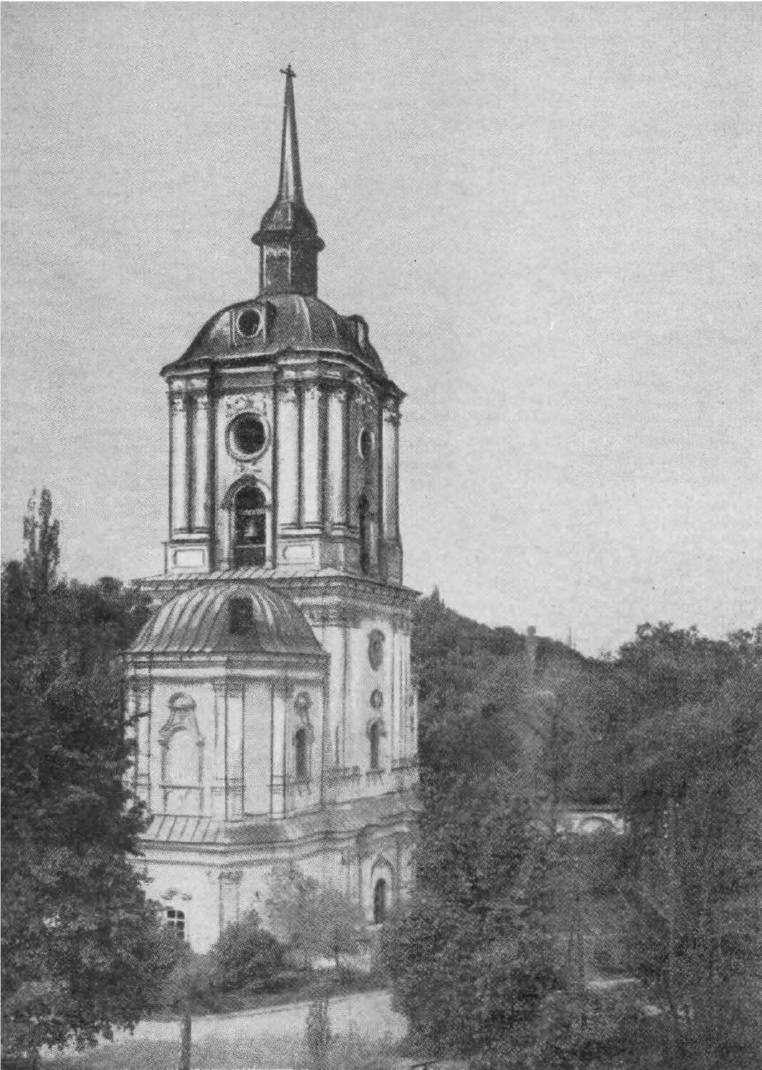
\includegraphics[width=\linewidth]{chast-zmiy/kurilo/kyr-kolo.jpg}

\textit{Колокольня архитектора Григоровича-Барского, простоявшая по 1937 год.}
\end{center}
\vspace*{\fill}
\newpage

Что тут было до монастыря? 

В книге Брайчевского «Когда и как возник Киев» 1964 года приводятся, со ссылкой на В. Д. Дяденко, следующие краткие сведения:

\begin{quotation}
Остатки городища чернолесской эпохи открыты на территории больницы им. Павлова [...]. Оказывается, древнерусское городище (к которому относится и сохранившаяся до наших дней Кирилловская церковь) возникло на месте более древнего городища начала раннежелезного века. В 1959 г. здесь при земляных работах были обнаружены следы жилищ полуземляночного типа; найдены обломки характерной керамики чернолесского типа, а также – фрагменты каменных зернотерок. Культурный слой, в частности, был обнаружен и под фундаментами Кирилловской церкви.
\end{quotation}

Кто возвел церковь?

В давнее время, церковь эта существовала не сама по себе, а в составе одноименного монастыря. Максимович посвятил ей статью «О создании киевской церкви св. Кирилла», где собрал доступные сведения и пришел к выводу, что церковь построена была княгиней «Марией Мстиславной, женой Всеволода Ольговича, дочерью Мстислава великого, внука Владимира Мономаха», что согласуется с летописью.

Закревский тоже приводит цитаты, и по ним получается, что монастырь основал Всеволод, отец Святослава.

Максим Берлинский, зная об упоминаниях монастыря в летописи, вразрез с нею предположил, что монастырь так назван по имени некоего Кирила, который способствовал восстановлению монастыря после «неистовства Батыева». При этом, полагал Берлинский, Кирил победил в окрестном лесу шайку разбойников, что и стало основанием легенды о Кириле Кожемяке и змие, «коего пещеры и теперь в лесу видны». Тоже подкованный в летописях, Закревский в дополнение кратко приводит содержание легенды, где Кирило Кожемяка сражается со змеем, побеждает его и в память о победе своей строит монастырь, «названный по его имени Кирилловским». Закревский также сообщает о множестве «Кирилловских пещер» и соотносит легенду о Змие с одной из них. Оставим же вопрос возникновения монастыря и церкви открытым.

%Вообще первое упоминание о Кирилловском монастыре в летописи таково, за год 1171:

%\begin{quotation}
%Сняшася братья Вышогороде и пришедше сташа на Дорогожичи под святым Кюрилом.
%\end{quotation}

%Теперь про Дорогожичи. Есть в Лаврентьевском да Ипатьевском списках за, по принятой датировке, 980 (6488) год:

%\begin{quotation}
%Стояше Володимер обрывся\footnote{Выкопал там защитный ров.} на Дорогожичи, межю Дорогожичем и Капичем, и есть ров и до сего дне.\end{quotation}

%Обратим внимание на уточнение – между Дорогожичем и Капичем. Капич – то же, что капище. Несколько позже, за 1146, читаем в Ипатьевской летописи:

%\begin{quotation}
%ту побеже Игорь и Святослав в слудовы Дорогожьчьския [...] и вбеже Игорь во болото Дорогожичьское и угрязе под ним конь
%\end{quotation}

%И за 1161 год такое описание:

%\begin{quotation}
%Перебредше Днепр, у боженки, и пойде полки к Киеву, и пришеди ста на Болоньи в лозах, противу Дорогожичу, иде к Подолью, а Ростислав стояше подле столпье (бревенчатой ограды); загорожено бо бяше тогда столпием от Горы, олы и до Днепра.
%\end{quotation}

%«У боженки» что значит? Боженка – божница, капище. А на каком берегу, левом или правом? Не сказано. Днепр перебрели у боженки. Брод там был. Брод, бродить, брести, перебрести – один корень. И перейдя через брод можно было, двинувшись в сторону Киева, добраться до Болонья-Оболони, и стать напротив Дорогожичей. Сие дает основание полагать, что тогда в пределы Дорогожичей люди включали и холм, на котором стоял Кирилловский монастырь.

%А боженка и Капич – одно ли урочище? Одно, если боженка – на правом берегу. Капич – точно на правом. Раз Капич и Дорогожичи – смежные, а боженка и Дорогожичи тоже смежные, значит боженка равняется Капичу. Ежели это справедливо, то Капичем, боженкой, некое место у Днепра близ переправы слыло по меньшей мере 1161 летописный год.

%Если же Боженка – на левом берегу, получается, что Капич – отдельное урочище близ Дорогожичей, и Боженка к Капичу не относится. В таком случае Капичем мог называться Бабий яр, где, как я предполагаю, на холме стоял идол, «баба».

Долгое время монастырь занимал всю местность, где теперь корпуса психиатрической больницы и церковь. В конце 18 века у монастыря отобрали земли, а затем и сам монастырь был упразднен, осталась только церковь, трапезная да колокольня (снесли в 1936 – помешала!), а в остальных зданиях поместились Кирилловские богоугодные заведения, где еще тогда, кроме прочего, устроили больницу «для умалишенных». Из нее и выросла, в 1920-30 годах, пресловутая психушка Павловка. 

Что же было на месте холма, когда там не стоял «святой Кюрила»? Помимо краткого сообщения Брайчевского про «остатки городища чернолесской эпохи», от которых ни холодно, ни жарко, сведений мало.

Там где на холме, будто крепкий гриб, растет сама церковь, была одна или несколько пещер, а скорее – целая сеть подземных ходов, пронизывающих гору.

Сементовский в 1864 году полагал, что у истоков Кирилловского монастыря стояли отшельники, обитавшие в пещерах. Дескать, в конце 11 или начале 12 века инок Кирилл вырыл там «пещерную келию». Закревский считал это выдумкой Сементовского.

%В конце 1880-х где-то около храма провалилась земля и открылся подземный ход. Туда проник служитель церкви Кулиш и увидел гробы в нишах, перпендикулярных коридору. Позже лаз в пещеру был засыпан.

Газета «Киевлянин» в нумере 238, 1909 года, напечатала статью Л. Зимина «Кирилловская обитель», откуда выпишу всё важное, опуская общеизвестные сведения про историю церкви и тому подобное.

По ходу будем разбирать прочитанное.

\begin{quotation}
В субботу, 15 августа, архитектор Д. В. Милеев, под наблюдением которого проводятся археологические раскопки в усадьбе Десятинной церкви, супруга его, большая любительница археологии, прив. доц. В. Г. Ляскоронский, подполковники Б. С. Стеллецкий и М. К. Дитрихс и автор настоящей заметки совершили поездку для исследования обнаруженной возле Кирилловской церкви пещеры с погребениями да кстати лишний раз осмотреть и самую церковь.

Кирилловские богоугодные заведения находятся на краю города на отдельном холме, который одним оврагом\footnote{Репяхов яр.} отделяется от Киева, другим\footnote{Бабий яр.} от Копылова.

Лукьяновско-Кирилловская линия трамвая чуть ли не самая интересная в Киеве. С нагорной ее части открываются широкие и живописные виды, особенно на долину Днепра; большая же часть линии пролегает по склону большого оврага\footnote{Репяхов яр.}, так что с одной стороны вы видите крутой откос горы с жалкими хатами наверху, а другой обрывистый склон оврага, сильно разветвляющегося и далеко вдающегося в гору; по дну оврага, по зеленому бархатному ковру течет довольно большой ручей, к которому в разных местах присоединяются меньшие.

В одном месте трамвай проходит через небо\-льшое ущелье.

В горах кое-где чернеют пещеры; одна из них очень просторная, эти пещеры мы пока еще не осматривали.
\end{quotation} 

Пещеры! Где же именно они были, как и когда сгинули? «Кое-где» мало что проясняет.

Зимин описывает поездку на трамвае, и это дает зацепку, что речь может идти только о той части Репяхова яра, по которой проходил маршрут – склон южного отрога и лежащий к северу от него отрезок яра, где оба отрога, составляющие этот громадный овраг, уже соединились у развилки при остром клинообразном мысе.

Серпантин дороги вдоль берега яра, трамвай да ручей – известный вид на дореволюционных открытках. Современные краеведы окрестили это место «Киевской Швейцарией», а книги и статьи переполнены ошибочными сведениями о том, что трамвай шел по улице Макаровской.

На деле же трамваи маршрутов 18 и 20 ходили непосредственно в яру (нисходя в него), под Макаровской, что на западном гребне отрога Репяхова яра. Маршрут 18-го трамвая, в некотором переложении на современность, был таким: нынешний сквер с фундаментом церкви св. Федора (на пересечении Овручской с Багговутовской) – Овручская – Нагорная (Подольского спуска не было), затем по Врубелевскому (тогда Макаровскому) спуску в Репяхов Яр до Кирилловской площади, и назад по яру же и через Пугачева да Багговутовскую обратно к церкви св. Федора. С течением времени маршрут несколько менялся, но первоначальный был именно таков.

Ручей в яру сохранялся до 1950-х, в нем даже водилась мелкая рыба. На одном из склонов местные жители помнят несколько пещер, а про семидесятые годы рассказывают, что в конце Ново-Макаровской улицы, на пригорке обитал отшельник, старик. Он выстроил себе приземистую хижину из бревен и разводил пчел.


%А в 1913 году существовал еще длиннющий маршрут 20, от Думской площади («Майдан»), по Большой Житомирской, Дорогожицкой, Овручской, затем повторявший часть 18-го и следующий еще далее Куренёвкой по улице Кирилловской.

%r03.jpg
%r04.jpg

%r01.jpg

%r07.jpg
%r08.jpg

\vspace*{\fill}

\begin{center}
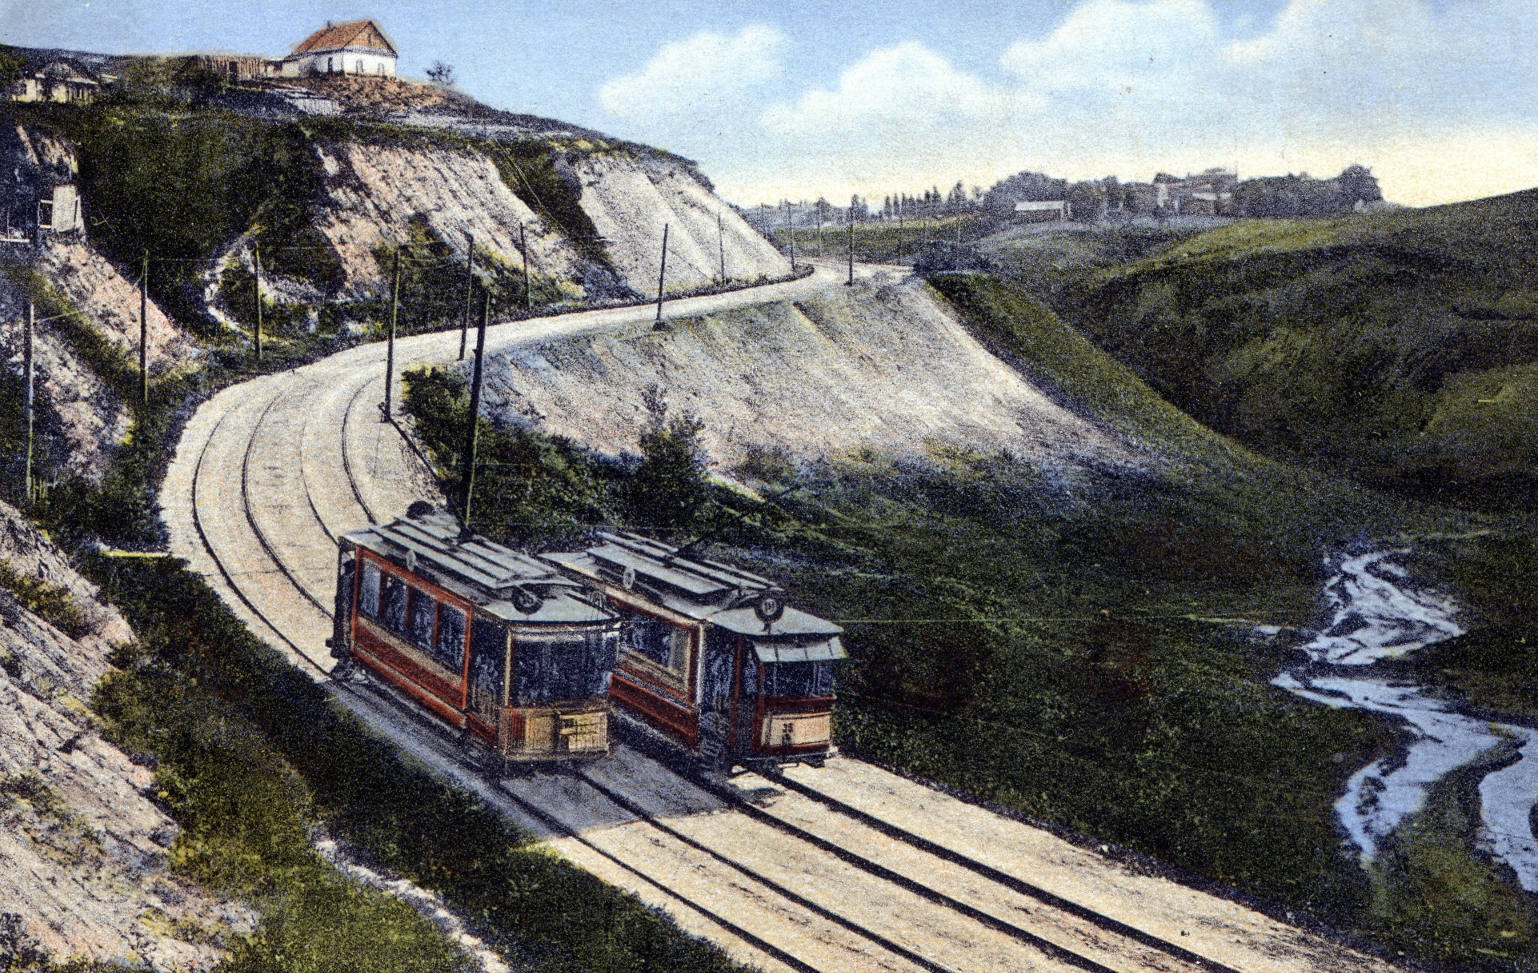
\includegraphics[width=0.90\textwidth]{chast-zmiy/kurilo/s-r09.jpg}

\textit{Вид снизу вверх, Кирилловская церковь позади фотографа справа.}
\end{center}

\vspace*{\fill}


\begin{center}
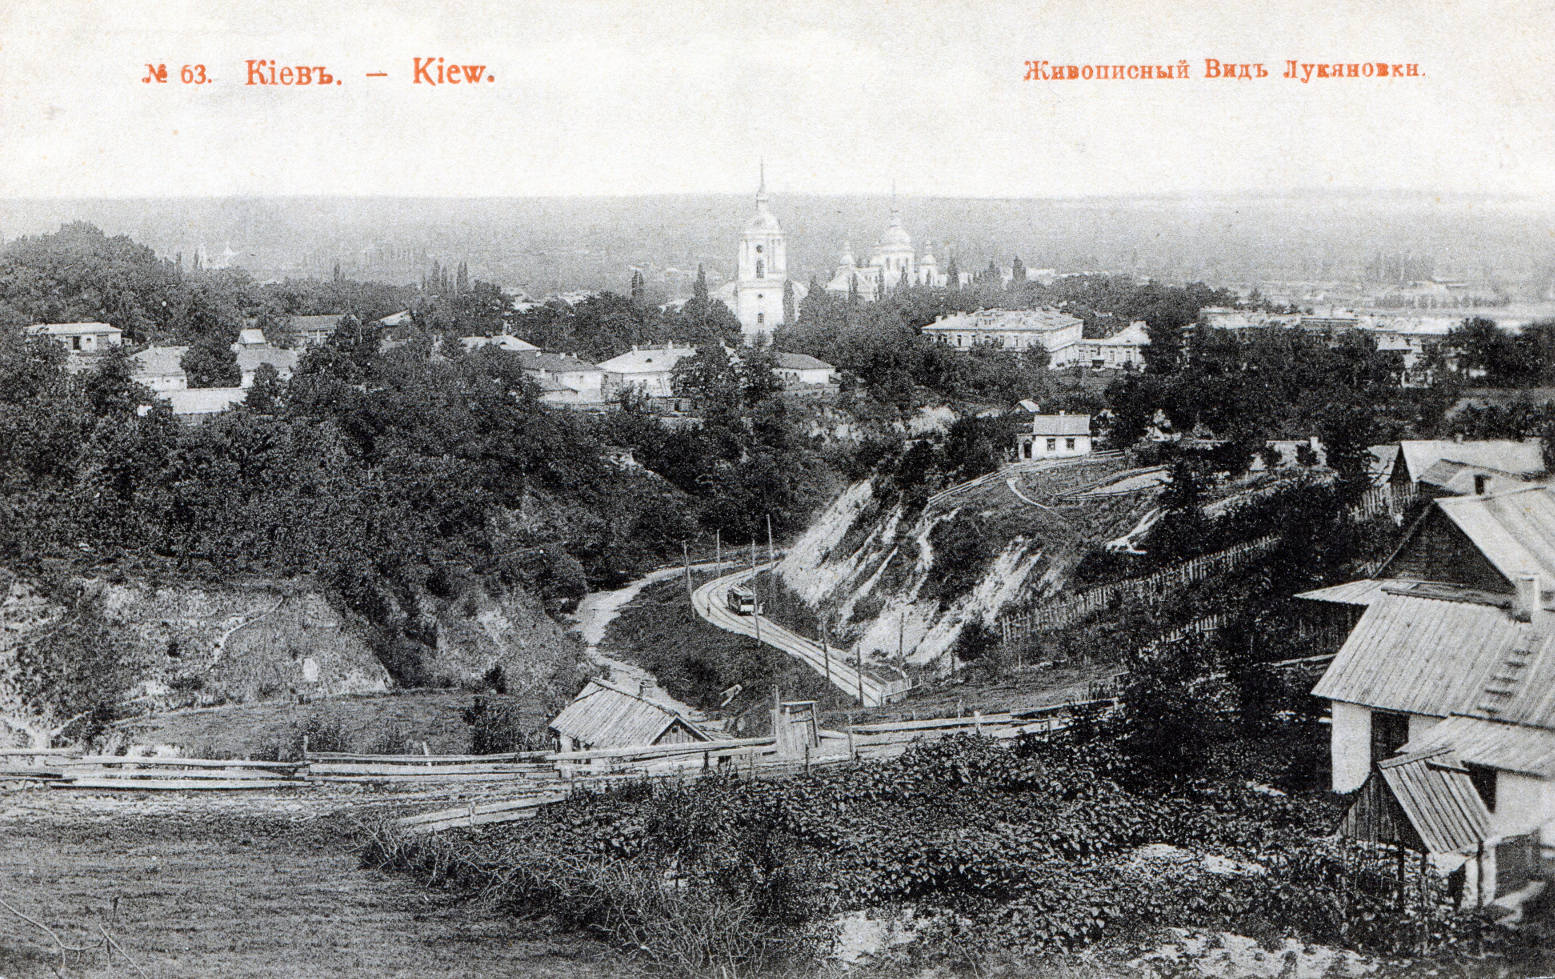
\includegraphics[width=\linewidth]{chast-zmiy/kurilo/s-r02.jpg}

\textit{Вид сверху вниз, в сторону Кирилловской церкви с колокольней. Дореволюционная открытка.}
\end{center}

\vspace*{\fill}

\begin{center}
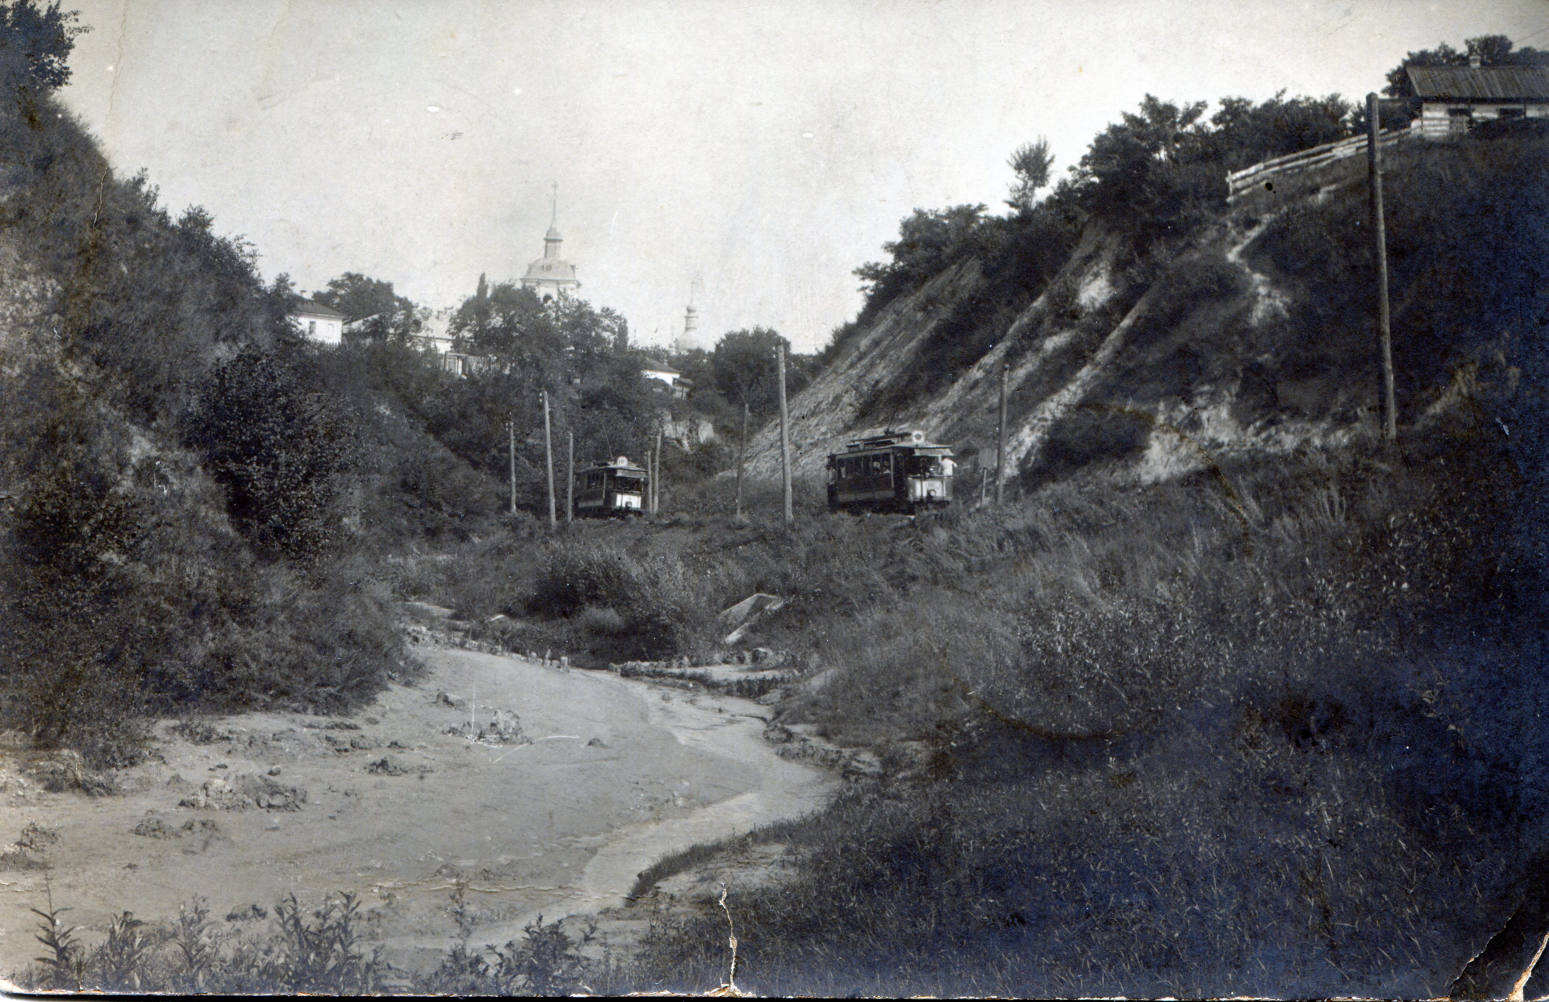
\includegraphics[width=\linewidth]{chast-zmiy/kurilo/s-r05.jpg}

\textit{Старинный снимок сделан в самом яру.}
\end{center}

\vspace*{\fill}


%\begin{center}
%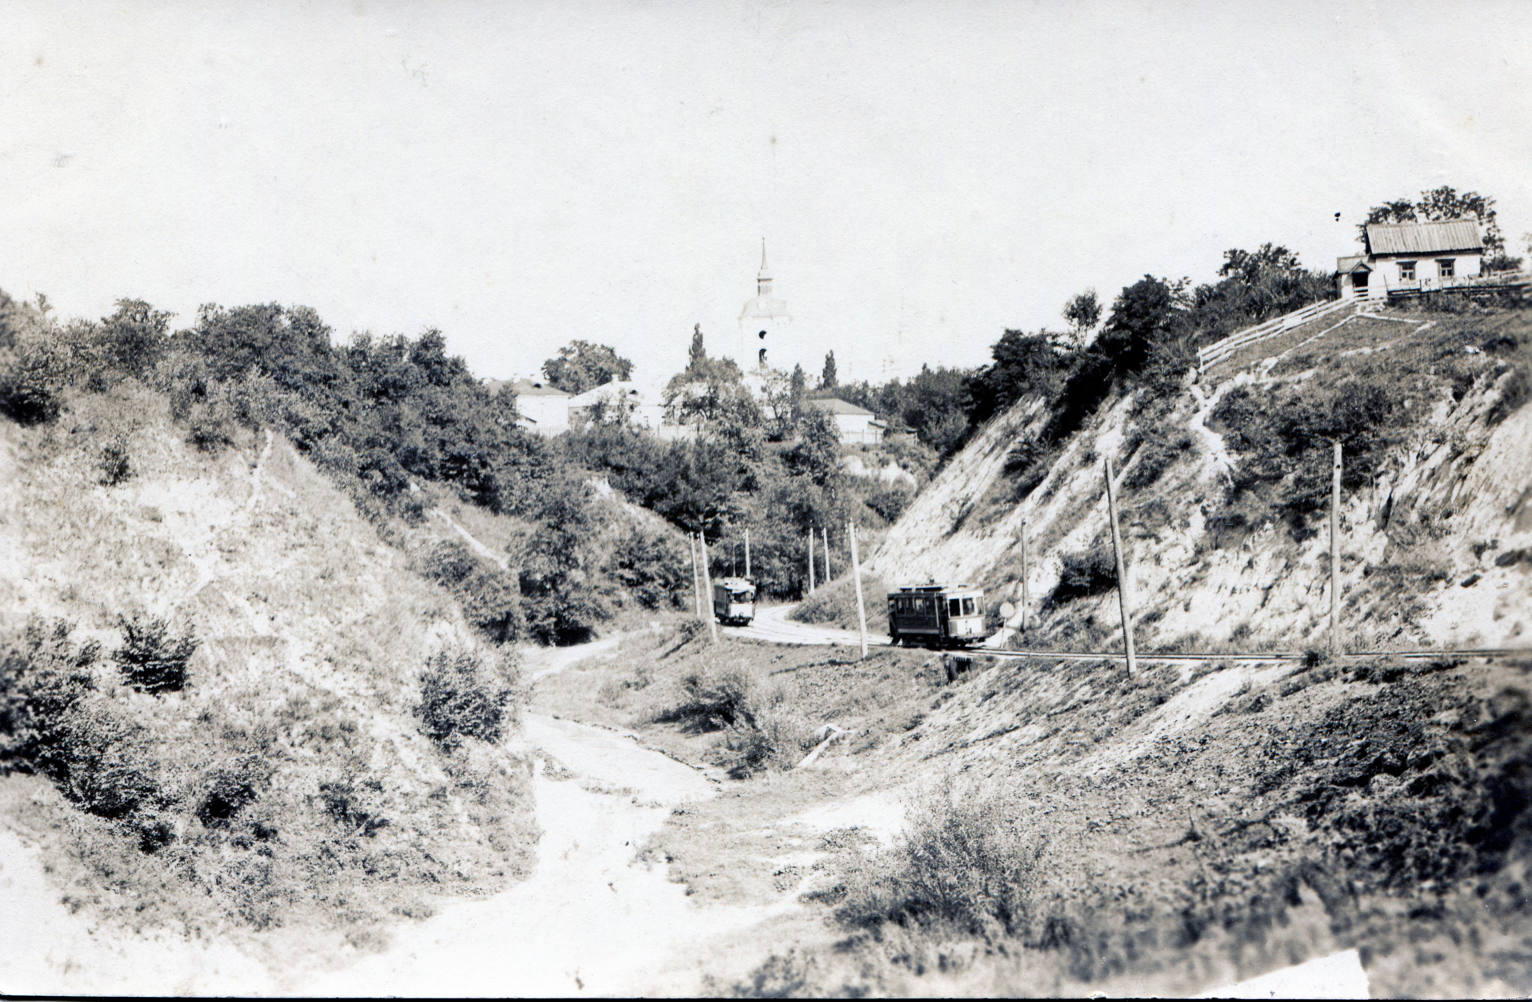
\includegraphics[width=\linewidth]{chast-zmiy/kurilo/s-r06.jpg}

%\textit{И сей тоже.}
%\end{center}
%\vspace*{\fill}

\begin{center}
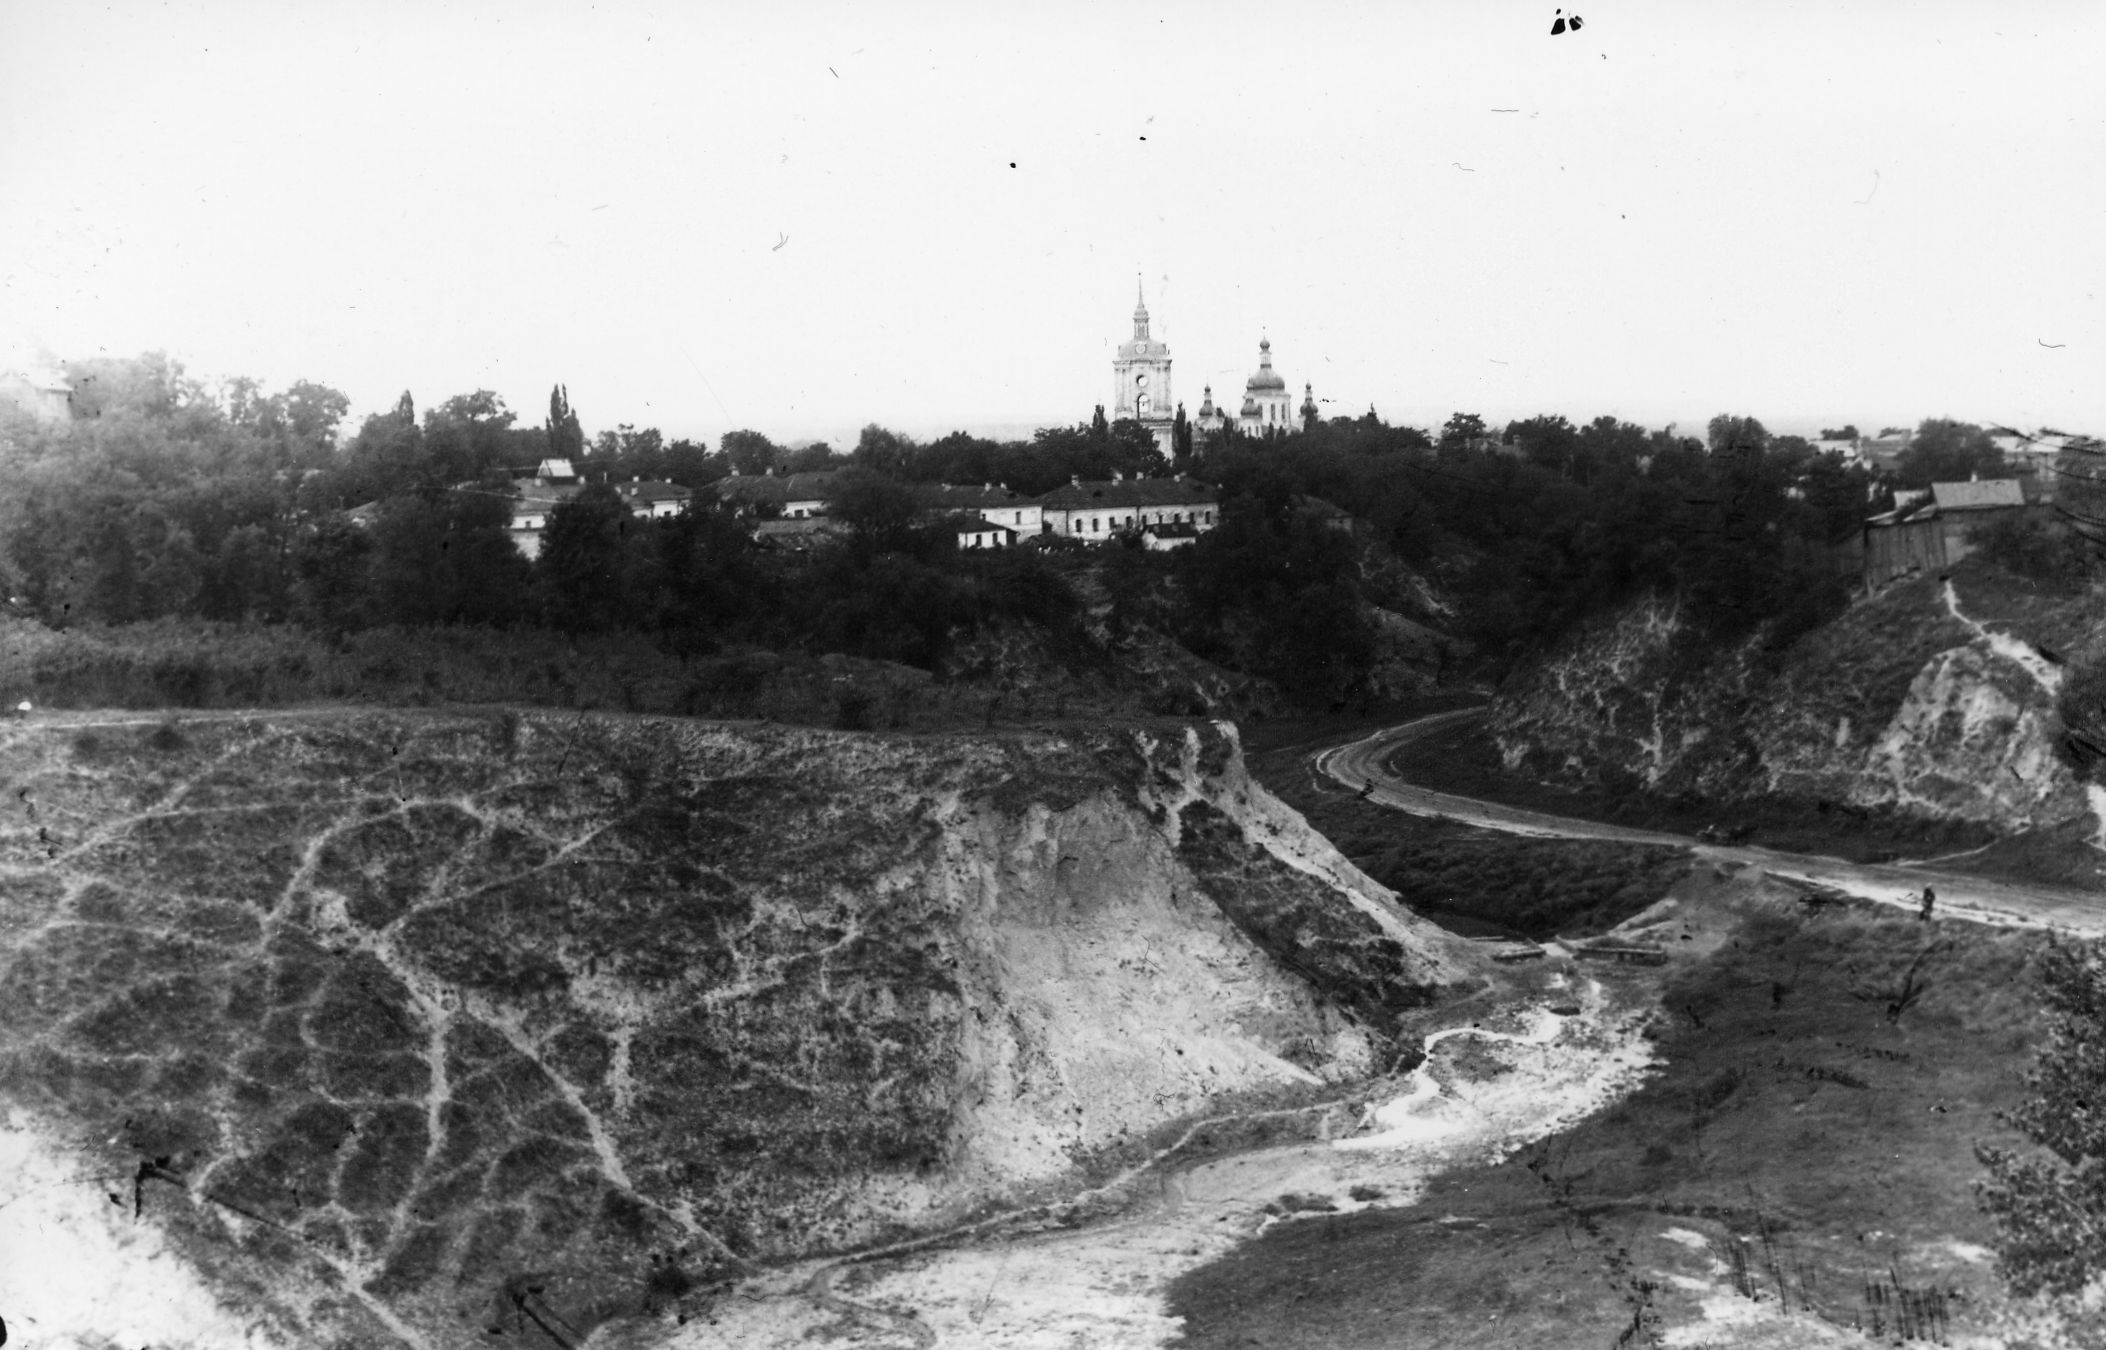
\includegraphics[width=\linewidth]{chast-zmiy/kurilo/rep-14.jpg}

\textit{Дореволюционный снимок. Трамвай еще не ходит.}
\end{center}

Всё то, что показано на открытках и фотографиях, нынче выглядит совсем иначе. Часть Репяхового яра занимают бесконечные гаражные кооперативы, их остатки да подобные проявления человеческой цивилизации. С ними можно познакомиться, спускаясь по выморочной Макаровской улице и левее, левее. Отовсюду торчат бетонные, кирпичные фундаменты, ржавая арматура, в земле зияют провалы, и всё это буйно заросло деревьями, бурьяном и щедро украшено россыпями битого стекла – ах, как блестит оно на солнце!

Вдоль Макаровской в сторону Репяхового яра отделяется дорога с красивым названием – Врубелевский спуск. Между гаражей и замусоренных склонов, дальше уводит он в места, где и днем всюду чудятся разбойники. Это здесь были проложены трамвайные пути. На некоторых отрезках спуск совсем непроходим – надо лезть в обход или перебираться по краешку обвала.

Вдоль южного отрога Репяхового яра, Врубелевский спуск нисходит по зарослям репейника ко дну самого яра чуть восточнее места соединения двух главных, громадных оврагов, составляющих Репяхов яр в виде упавшей на левый бок, искореженной буквы «Y».

\begin{center}
\includegraphics[width=\linewidth]{chast-zmiy/kurilo/\myimgprefix IMG_20130915_143657.jpg}

\textit{2013. Начало Врубелевского спуска, наверху.}
\end{center}

По каждому из них протекает ручей. Как и овраги, оба ручья сходятся и далее текут уже вместе. Так было прежде, до вмешательства человека. Ныне часть вод загнана в пахнущий химией коллектор, а часть протекает поверхностью – у обочины и просто дор\'огой, вымощенной бетонными плитами от стройки, что ведется в дальней части одного из приярков. На плиты ручьем намыло богатую железными частицами, буроватую глину, в которой завелись микроскопические водоросли. Дорога пахнет морской капустой или речными водорослями, которые вытащены на сушу и сохнут в песке.

%На этой фотографии запечатлено место, откуда трамвай по террасе спускался в яр:

%\begin{center}
%\includegraphics[width=\linewidth]{chast-zmiy/kurilo/\myimgprefix IMG_20130915_144450.jpg}
%\end{center}

%\newpage

%И пара снимков 2013 года, уже на дне яра:

%\begin{center}
%\includegraphics[width=0.95\linewidth]{chast-zmiy/kurilo/\myimgprefix rep-05.jpg}
%\end{center}

%\begin{center}
%\includegraphics[width=0.95\linewidth]{chast-zmiy/kurilo/\myimgprefix rep-08.jpg}
%\end{center}

%\newpage


\begin{center}
\includegraphics[width=\linewidth]{chast-zmiy/kurilo/\myimgprefix IMG_20130915_144633.jpg}

\textit{2013. Дорога на дне яра.}
\end{center}

Со склонов сочатся ручейки и бегут между зарослей репейника. У обочины встречаются наполненные водой ямы, где видно относительно крупные водоросли, похожие на хвойные ветки. По склонам яра стоят, подпирая небо, громадные деревья – ивы с толстенными стволами, серебристые тополя. Некоторые деревья увиты лианами.

Сами склоны рассмотреть зачастую трудно из-за зелени, мокроты и нагромождений живых и сломанных деревьев. От голых склонов с фотографий 19 века не осталось и следа.

Такова местность, описанная Зиминым, сейчас. Продолжим читать его статью.

\begin{quotation}
В церковь мы прибыли в одиннадцатом часу утра; несмотря на большой праздник, молящихся было очень немного, да и те, судя по одежде, из больницы и богадельни. Находясь в мало населенной местности и не имея прихода, Кирилловская церковь является как бы домовой церковью при Кирилловских богоугодных заведениях и вместе с ними состоят в ведении Киевского губернского земства.
%\end{quotation}

%\begin{center}
%\includegraphics[width=\linewidth]{chast-zmiy/kurilo/\myimgprefix vidkyr.jpg}

%\textit{Дореволюционный снимок. Вид на Кирилловскую церковь со стороны низовья Бабьего яра, там где перекресток Кирилловской и Телиги.}
%\end{center}

%\begin{quotation}
Настоятель церкви был занят, единственный из служащих, видевших пещеру и погребения, некий Кулиш, ушел на курёневскую ярмарку, а смотритель зданий мог только приблизительно указать то место на склоне горы, где должен быть вход в пещеру.

Подполковник Дитрихс и я спустились и тщательно осмотрели весь склон у подошвы горы; нашли множество нор, из которых две своими размерами особенно привлекли наше внимание; пещеры же не нашли.

Смотритель послал разыскать Кулиша; мы же, ожидая его возвращения и окончания службы, расположились на травке под стеною храма, беседуя как о самом Кирилловском храме, так и о других памятниках старины. [...]

Последний раз Кирилловская церковь упоминается в летописи под 1231 годом, а затем до 1555 г. о ней нет никаких сведений. [...]

%Батый, разгромив Киев, почему-то не тронул Кирилловской церкви.

В 1555 году Сигизмунд II отдал Кирилловскую церковь со всеми имуществами, которые ей принадлежат, некоему Шавуле, предоставив ему те же права по отношению к церкви, какими пользовались его предки; в 1565 году имущества упраздненной Кирилловской церкви приписаны к Никольской церкви, которая находилась в киевском замке. [...]

И только в 1605 году известный ревнитель православия князь Острожский поручил игумену Острожского монастыря св. Креста Василию Красовскому восстановить Кирилловский монастырь и возвратить все имущества [...]

Кулиш с ярмарки не возвращался; терпение наше истощалось, и мы уже все компанией принялись за новые поиски\footnote{Давно пора, чем Кулиша ждать.}. Вышеупомянутые норы оказались ниже того уровня, где возможно было бы существование пещер; но там, где это возможно, ни нор, ни каких-либо иных признаков существования пещер не оказалось.

Нашли несколько кирпичей XVII века, вероятно обломки стены, часть которой сохранилась до сих пор, а часть, шедшая по краю горы, разрушена; фундамент ея в некоторых местах выступает наружу.

Мы еще не закончили своих поисков, как нас пригласили к священнику. Он указал нам на краю горы, шагах в 45 к северу от храма место, где стояла часовня; возле нея, ближе к храму, находился морг, т.е. ледник для хранения мертвецов, а возле него образовался какой-то провал, в котором и обнаружена была пещера.

Кулиш проник в эту пещеру и по сторонам видел гробы в нишах, лежащие не вдоль пещерного хода, как в лавре, а перпендикулярно к нему. Кулиш прошел несколько сажен по направлению, как он думает, к северному входу в храм и, увидав толстые скрещенные балки, дальше идти не решился.

Было это лет двадцать тому назад, но до сих пор никто не счел нужным исследовать эту пещеру, и только теперь Б. С. Стеллецкий, прослышав о ней, организовал компанию для археологической разведки.

От часовни не осталось и следа, морг и провал засыпаны; все место сравнено с остальной площадью, на которой стоит храм; кроме того тут идет систематическая свалка для дальнейшего расширения площади.

Для того, чтобы на склоне горы открыть вход в пещеру, пришлось бы снять большой пласт и на довольно большом пространстве, так как точно место входа осталось неизвестным.

Поэтому решили сделать траншейку на пути от бывшего провала к северному входу в храм; траншейка, конечно, должна пересечь пещерный ход. Поручив это дело опытному рабочему, которого захватил с собой Д. В. Милеев\footnote{Рыть сообща было бы скорей, белоручки.}, мы тем временем решили осмотреть храм.

Пока ходили за ключами, священник указал нам место, где находилась трапезная церковь во имя св. Василия – это шагах в 40 к западу от храма; там сейчас клумба цветов. Священник говорит, что пол бывшего алтаря остался нетронутым; возможно что под престолом, как это обыкновенно делается, заложена ценная святыня.

Вокруг Кирилловской церкви было когда-то кладбище; один из надгробных камней еще и теперь лежит сверху; остальные, по словам священника, зарыты вдоль северной стены храма.

Проходя по этому месту, мы невольно обратили внимание на двери северного входа; в них щели пальца в два шириной, нижняя доска совсем вывалилась; в таком же состоянии оказались южныя двери; [...] 

Тем временем во дворе уже вырыта была траншейка, и некоторое время думали даже, что попали как раз на погребение; однако это не подтвердилось, и прощупывание почвы длинным железным стержнем тоже не давало никаких результатов.

Наконец, явился Кулиш и, по его рассказу оказалось, что траншею следовало рыть немного левее\footnote{Следовало дождаться Кулиша и тогда уже рыть траншею.}. Начинать новую траншею было уже поздно; пришлось поиски пещеры отложить до другого раза [...]
\end{quotation}

Компания посетила трехярусную колокольню 1748 года строения, третий этаж которой был поначалу деревянным, но сгорел в 1849 году, и его возобновили каменным.

\begin{quotation}
По обе стороны главного корпуса колокольни имеются пристройки; в одной из них находится лестница; сначала она широкая, заполняет всю пристройку, а выше заменяется двумя; одна ведет во второй ярус, где теперь помещается аптека Кирилловской больницы; другая тоже во второй ярус, в верхнюю часть его – на потолок больницы\footnote{Далее в статье речь идет о потолке аптеки, таким образом второй ярус был разделен на два этажа, один с аптекой, другой – помещение над нею.}. Над входом в помещение аптеки имеется чугунная доска с надписью, свидетельствующая о том, что в 1760 году игуменом Феофаном Желтовским здесь была устроена церковь во имя Благовещенья. [...]

На третий ярус ведет узкая каменная лестница, заключающаяся внутри стены. Пол третьего яруса страшно ветхий, в одном месте и притом как раз около колоколов большая дыра; говорят, что зимой здесь бывает по колено снегу, который, конечно, забивается под пол на свод второго яруса, где потом тает, проводя сырость [...]

Есть еще деревянная лестница на самый верх колокольни, но смотритель не советовал взбираться туда, вследствие ветхости и лестницы, и помоста. 

Колоколов немного и самый большой из них очень невелик; видно, что колокольня рассчитана на гораздо большую тяжесть.
\end{quotation}

Затем любители старины отправились исследовать некую пещеру неподалеку:

\begin{quotation}
Осмотрев колокольню, пошли к пещере, находящейся, за кладбищем версты за полторы от церкви\footnote{Около 1,6 км.}.

На вершине высокого мыса, называемого местными жителями Курганом, находится довольно большая яма, а в ней нора, сразу уходящая вниз на неизвестную глубину; 

в нескольких шагах от нея на склоне горы другая таких же размеров, но уходящая в гору горизонтально; с другой стороны Кургана еще одна, широкая, просторная.

Так как забираться в пещеры без огня не было никакого смысла, то послали в лагери\footnote{Вероятно, военные лагеря, между речкой Сырец и верховьем Бабьего яра. Окрестности улицы Вавилона и примыкающего к ней отрезка Щусева. Туда можно добраться как от Репяхового, так и Бабьего яров. Думаю, от Кургана до лагерей было ближе, чем к Кирилловской церкви, раз послали за свечами в лагеря.} за свечами, а тем временем Д. В. Милеев, подполковник Дитрихс и я, в сопровождении сторожа, спустились на дно оврага, где протекает довольно большой ручей; почти на каждом шагу встречаются родники; один из них, появившийся только в этом году, довольно большой; вода этого родника чистая, холодная, с сильными минеральными примесями.

Ручей, размывая почву, обнажил толстый пласт дерева; в некоторых местах сохранилось слоистое строение, и там, где пласт особенно подвержен влиянию воды, слои легко отделяются друг от друга; в иных же местах попадаются уже не слоистые, а однообразные строения куска (угля) с ясными, однако, следами сучьев.

Мы захватили образцы для того, чтобы показать специалистам по ботанике и геологии, не имеем ли мы дело с остатками первобытных лесов.

Когда мы поднялись из оврага, были принесены уже и свеча, и лампа.

Большая пещера особого интереса не представила; будучи освещена внутри, она вся видна от входа; никаких ходов в стороны нет; свод в ней сырой; очевидно над ней находится водоносный слой.

Другая пещера оказалась интереснее. Пробраться в нее можно только ползком, но в неско\-льких шагах от входа она уже так высока, что рукой нельзя достать ея свода.

Кроме того, подполковник Дитрихс прошел по ней прямо тридцать шагов, повернул налево, прошел еще 19 шагов. Дальше пещера поднимается, но сама становится ниже; по-видимому, она имеет другой выход, как так ощущается небольшой сквозняк, но вместе с тем лампа сильно портит воздух; 

опасаясь возможности взрыва, подполковник Дитрихс вернулся назад, решив в один из ближайших праздничных дней исследовать пещеру до конца с электрическом фонарем.

Пещера, по-видимому, посещается, так как стены ея исписаны, но подписей подполковник Дитрихс не разобрал. Говорят, что здесь искали клад. [...]

Третью нору не исследовали, так как стало темнеть. Следующая разведка должна дать более интересные результаты, так как займемся исключительно пещерами и исследуем их до конца.
\end{quotation}

В номере 248 за 1909 год «Киевлянин» напечатал еще одну заметку про Кирилловскую церковь и находящиеся рядом пещеры. Почитаем.

\begin{quotation}
Внимание комиссии\footnote{Ее состав: Б. С. Стеллецкий, Дитрихс, Ляскоронский, Д. В. Милеев.} обратила на себя находящаяся у северной стены древней церкви пещера, о которой раньше археологи не знали. 

Было известно о существовании пещеры на южной стороне холма, на котором расположена церковь. Лет 30 тому назад на этом месте образовался провал и один смельчак задумал спуститься в пещеру, в которой предполагались сокровища. Смельчак, спустившийся по веревке, за которую держались несколько человек, своего предприятия не довел до конца в виду огромной глубины. Исследованием новооткрытой пещеры и думает заняться комиссия\footnote{Идет ссылка на Киевские Вести 19 августа, номер 220 и Спб. Ведомости 23 августа, номер 188.}.
\end{quotation}

Очень неоднозначно написано. По смыслу вроде бы можно сопоставить «смельчака» со служителем церкви Кулишом из предыдущей статьи. Однако в ней не было подробностей про спуск на веревке, и Кулиш лазал в пещеру, ход куда открылся «шагах в 45 к северу» от храма, а тут речь идет про «южную сторону холма».

Прикидывая на местности, 45 шагов на север – там действительно крутой северный склон горы, с каменной лестницей за зданием бывшей прачечной, ныне морга. А южная сторона горы – метрах в двухста от церкви, склон уже Репяхового яра.

Поэтому я не понимаю, то ли написано о двух разных пещерах – северной и южной, то ли спутаны стороны света и вместо «южная сторона холма» следует читать «северная», тогда всё становится более ладным. Дескать, лет тридцать назад открылась пещера на северном склоне, на неё-то сейчас и обратили внимание археологи. 

Иначе придется предположить, что была еще какая-то пещера на южном склоне, куда 30 лет назад спускался на веревке не Кулиш, а какой-то другой смельчак.

Но на карте Хвойки, которую я приводил в главе «Кирилловская стоянка», создатель ея обозначил таки две пещеры возле церкви. Одну пещеру у северной стороны церкви, другую подле, примерно, восточного угла горы, направленного к стадиону. О последней пещере все источники молчат.

Еще более примечательно, что карта Хвойки опубликована в 1899 году, а мы разбираем статьи 1909-го. И вот Зимин, Дитрихс, Стеллецкий, Ляскоронский, Милеев в первой статье разводили руками и заставляли рабочего копать в ошибочном месте, и ждали Кулиша, а у Хвойки уже за десять лет до того там указаны целых две пещеры – одна из которых, судя по всему, и есть та самая «северная».

\begin{quotation}
6 сентября члены киевского отдела Императорского военно-историческаго общества Б. С. Стеллецкий, М. К. Дитрихс, проф. В. В. Завитневич и некоторые другие лица вновь совершили поездку для исследования кирилловских пещер. Пещеру, находящуюся возле самой церкви, вследствие отсутствия архитектора Д. В. Милеева и В. В. Хвойка, не раскапывали;
\end{quotation}

«Возле самой церкви» – вероятно, речь идет о той самой «северной» пещере, куда лазал Кулик. Отметим еще, что Хвойка и Милеев не явились. Так и неясно, проводилось ли исследование пещеры в 1909 году. 

\begin{quotation}
ограничились лишь пещерой, находящейся в так называемом Кургане за Кирилловским кладбищем. Пока рабочий под наблюдением Б. С. Стеллецкого расчищал вход в пещеру, остальные члены компании спустились на дно оврага, чтобы показать проф. В. З. Завитневичу те пласты дерева и угля, о которых я недавно сообщил в «Киевлянине». Проф. Завитневич очень заинтересовался как этими пластами, так и вообще слоями почвы, которые здесь выделяются очень отчетливо, и захватил образцы для более детального исследования.

Когда вход в пещеру достаточно расчистили, М. К. Дитрихс и я, в сопровождении одного рабочего, вооружившись лопатами и электрическими фонарями, проникли в пещеру; вскоре присоединился к нам и проф. В. З. Завитневич.

Сначала идет коридор, немного лишь заворачивающийся вправо, длиною 20 3/4 арш.\footnote{14,76 метра.}; по сторонам его попадаются ниши; некоторые из них настолько велики, что в них свободно может спрятаться человек. На 20-м аршине отходит ветвь влево, тоже немного заворачивающаяся в правую сторону, а в общем составляя с первым коленом угол в 50 градусов. Все протяжение второго колена около 9 аршин\footnote{6,4 метра.}.

На шестом аршине опять влево почти под прямым углом идет новый, короткий, всего около двух аршин, ход, который приводит в небольшую овальную пещеру; из нее во второе колено коридора пробито окно, вершков 5\footnote{22 сантиметра.} в диаметре.

Коридоры настолько узки, что оба плеча трутся об их стены; высота же их крайне различная. В некоторых местах насилу достаешь потолок рукой, в иных и особенно в конце можно пробраться только ползком; не только разминуться с кем нибудь, но и самому повернуться невозможно.

Объясняется это тем, что пол пещеры – наносный или позднейшие раскапыватели, ленясь удалять землю наружу, нагребли бугры по дороге, или вода их намыла, а может быть, действовали обе причины.

Раскапывая пол пещеры, находили твердый грунт лишь на глубине аршина и более. Когда ударяли о пол в конце второго коридора, то слышался гул, указывающий на пустоту под полом. Пол в самой пещере очень мягкий и при раскапывании обнаружен, как будто, ход вниз и обратно, в роде как бы второй или, вернее, подвальный этаж коридора; гул этот можно было объяснить еще и иначе: верхний слой пола утоптан, а ниже он сравнительно, рыхлый, следовательно более пустой.

Против вышеупомянутого окна, в правой стене коридора имеется низкая, но широкая ниша, а в ней уходящий вглубь рукав, в который можно только просунуть руку; дальше он заворачивает влево; такой же рукав есть рядом с нишей и в некоторых других местах.

Когда немного раскопали нишу, то в ней оказался еще один такой рукав. Задняя стена и потолок ниши были обмазаны известью, а на дне ея глина носит следы угля; очевидно, это был очаг, а рукава служили дымовыми трубами и вообще предназначены для вентиляции. Вероятно они и сейчас имеют выход наружу, так как воздух в пещере, несмотря на продолжительное пребывание в ней трех и четырех человек, оставался свежим. Вероятно, отверстия этих отдушин засорились, так что глаз не замечает их.

Мы нашли одно отверстие, но по-видимому, отдушина засорена где-нибудь внутри, потому что ни звук, ни свет внутрь пещеры не проходят. Присутствующие наверху кургана отчетливо слышали, как копались внутри пещеры. 

На дне только что упомянутой ниши оказалось еще углубление яйцевидной формы, тоже вымазанное довольно толстым слоем извести; кроме того, тут же попадаются комочки извести, напоминающие фигурки различных животных; некоторые из них, будучи ветвисты, все же плотно приходятся друг к другу.

Пещера находится в лесе; стены, свод, а также и пол ея, где нет наносной земли, настолько прочны, что весьма нелегко поддаются саперной лопате и весьма острому железному щупу. Если удалить наносную землю, то пещера, т.е. свободное пространство в конце коридоров, окажется довольно просторной, но удалять землю надо от самого входа, что потребует много времени.

Поэтому, осмотрев по верху в соответствующем направлении коридоры и видя, что яма с новой в вершине кургана приходится над пещерой, решили проникнуть в пещеру с этой стороны, надеясь, что это будет скорее, чем прочищать все коридоры. Однако, здесь нора сразу идет вниз и, по-видимому, на большую глубину, так что потрудившись до самого вечера, мы все-таки не достигли пещеры. 

Хотя, таким образом, окончательно расследовать пещеру не удалось, но открытая ниша, вымазанная известью, с явными признаками очага, с углублением, имевшим, очевидно, какое-то специальное назначение, а также несколько запутанные ходы, окно из пещеры в коридор, – все это показывает, что пещера выкопана не простыми кладоискателями; они могли только испортить ее последующими раскопками. (Наибольшее подозрение со стороны проф. В. З. Завитневича падает на известного генерала Багговута и жену его).

План пещеры очень близко подходит к плану леваго края Дальних пещер в Лавре, если смотреть от входа в пещеры. Надписи на стенах пещеры не дают никаких сведений, которые свидетельствовали бы о времени открытия ея; впрочем, разбирать все из требует слишком много терпения и хорошего освещения\footnote{Нигде более сведений о надписях, да и о самом Кургане, я не нашел.}.

Хорошо утоптанный насыпной пол показывает, что пещера посещается давно; в одной нише найдена визитная карточка некоего Ренского. На этот раз пещера заинтересовала нас еще более, чем в предыдущий, и мы, конечно, еще вернемся к ней\footnote{Заманчиво полагать, что в «Киевлянине» есть продолжение, однако я не знаю, в каком номере его искать.}. 
\end{quotation}

Поначалу я был знаком только с последней статьей, и не знал, что в первой указано расстояние до Кургана – полторы версты. Меня начало мурыжить, как же найти этот Курган. Я стал прикидывать.

Имелись ориентиры – Кирилловское кладбище да упомянут овраг: «Пока рабочий [...] расчищал вход в пещеру, остальные члены компании спустились на дно оврага». Значит, Курган с пещерой был около края оврага, причем в таком месте, где участники экспедиции, не скалолазы, могли слезть на дно.

Вдобавок меня сбило с толку сообщение о пещере в «южной стороне холма». Не ведая о первой статье, я как один из вариантов рассматривал, что пещера, куда лазал «смельчак» – та же, которая «в Кургане», и если это так, то Курган следовало искать в Репяховом яру. Ведь Кирилловское кладбище занимало поверхность горы на запад за Кирилловским монастырем, северной стороной выходя на Бабий, а южной – Репяхов яр. 

Прежде поисков Кургана, мы просто искали пещеры в Репяховом яру. В ходе съемок «Киевской амплитуды» и мной отдельно был исследован западный склон к западу от Макаровской улицы по дорогу на дне яра, и бегло осмотрена часть противоположного склона общего отрога. Пещер мы не нашли. Сложность местности, а заодно вмешательство  человека, существенно затрудняют дело.

Краеведческая вылазка вдоль южной части холма, на котором стоит Кирилловская церковь и больница, в июле 2014 года, когда мы пытались найти «местность Курган», принесла некоторые плоды.

Пробиваясь по краю яра вдоль забора, не доходя до свалки рядом с психбольницей, эдак по координатам 50°28'48.33"N 30°28'15.68"E, мы нашли вертикальный ход в земле, метра два глубиной, уходящий потом в сторону. Спускаться без каких-либо приспособлений туда не рискнули. Я порывался, но меня отговорили, мол, можно провалиться. Земля, а точнее глина внизу была рыхлой, лежал какой-то большой кирпич или камень. Хотелось думать, что это вход в пещеру, найденный «смельчаком» (мы еще не знали о первой статье Зимина), но про ту пещеру сказано, что «открылся провал», а здесь мы столкнулись с тщательно выкопанной шахточкой, причем в месте, куда очень трудно добраться с любой стороны.

\begin{center}
\includegraphics[width=\linewidth]{chast-zmiy/kurilo/\myimgprefix rep-IMG_3887.JPG}
\end{center}

Вниз по отвесному почти склону тянулась великанская борода мусора, двигаться назад в сторону Кирилловской улицы – сложно и долгонько, путь к окраине Павловки преграждают непреодолимые кусты и забор, а если продираться дальше с большой осторожностью, попадаем на свалку.

Ход был вырыт чем-то небольшим вроде саперной лопатки, потому что большой лопатой там не размахнешься. Следов выброшенного грунта снаружи не замечено, возраст раскопа определить трудно. Если там и лежали прошлогодние листья, то их присыпало землей. Форма хода – квадрат со сглаженными углами, если я спущусь, то подняв руки, достану до краев ямы, но широко расставить руки в стороны не смогу – узко.

Неясно, как далеко идет от дна горизонтальный ход. По виду, я бы мог засунуться туда ползком на спине, ногами вперед, никак иначе.

Продвигаясь от свалки\footnote{Кстати, в конце 1930-х свалка была и где-то на улице Макаровской, а это значит, что часть склона Репяхового яра, где могли быть пещеры, оказалась засыпана еще тогда.} (где я удачно наступил на шприц и пробил через кроссовок ногу) в неопределенном направлении, мы вышли к полукруглому тупику оврага близ недостроенного здания Института социальной и судебной психиатрии и наркологии.

Там, в тупике, странное место – непонятные деревянные сооружения, на суку дерева висел череп коровы, а склоне слева темнело несколько полузасыпанных пещерок. Конец просматривался во всех, кроме одной, где жили маленькие ёжики. Может раньше туда мог залезть человек, но теперь она слишком тесная. Мы скоро ушли, чтобы не беспокоить ежей – это их дом.

Выбравшись к заброшке института, мы продолжили исследовать тот же изъеденный оврагами южный склон горы, вдоль северного отрога Репяхового яра, на запад. По ходу однажды показалось, что там могла быть большая подземная полость с переходами, затем обвалившаяся. Так это или нет, проверить нельзя.

С тех пор прошло несколько лет. Поныне – пишу это в марте 2021 года – исследование Репяхового яра нами не завершено. В декабре 2019 года я нашел, вероятно, засыпанную пещеру на склоне над Репяховым яром, около заброшки Дурки, примерно по координатам 50°28'41.3"N 30°28'04.3"E. 

Непонятно, где – и в каком из яров – искать Курган, если следовать указанию, что он находился в полутора верстах от церкви.

Считайте, 1,6 километра. Если провести от церкви прямую линию на такое расстояние, то линия выйдет за пределы Репяхового яра аж до улицы Мельникова, и почти доберется до станции метро Дорогожицкой, если направить линию ближе к Бабьему яру. В окрестностях метро было верховье Бабьего яра, ныне засыпанное и плоское. А верховье состояло из мысов и приярков между ними. Вот координаты трех таких прежних мысов: 50°28'30.2"N 30°27'17.4"E, 50°28'30.6"N 30°27'10.1"E и 50°28'37.4"N 30°27'21.5"E, возможно один из них и есть бывший Курган, что-то подсказывает мне что последний, как самый высокий мыс. Если в статье нет ошибки с расстоянием.

Соберем сведения из обеих статей. Полторы версты от церкви. «За Кирилловским кладбищем» – а оно достигало нынешнего памятника Меноры, примерно возле которой отделялось от иудейского кладбища оградой. Высокий мыс, называемый «местными жителями Курганом». На дне оврага под мысом «протекает довольно большой ручей; почти на каждом шагу встречаются родники». Да, под всеми указанными мною выше мысами протекал ручей, но я не знаю, сколь обильным он был.

Под описание подходят, но если не брать в расчет полторы версты как точные данные, и Бабий, и Репяхов яры в тогдашнем их состоянии. Предположение, что в пещерах рылись Багговуты, дает небольшую зацепку, что местность ближе всё-таки к Лукьяновке, где у Багговутов была земля. Значит, кладём один довод на чашу весов в пользу Репяхового яра. 

Однако почему Зимин тогда не написал просто – по ходу трамвайной линии в яру?Возможно, Курган находился в стороне от этой линии, на запад. Возможно, с Курганом можно сопоставить мыс с Дуркой – от церкви до Дурки полверсты, а не полторы. Повторюсь – если принять за истину данное в заметке расстояние, то Курган был около метро Дорогожичи, иначе же где-то ближе к Кирилловской церкви.

А как насчет пещеры под церковью? Неясно, изучили ее в 1909 году или нет. В доступных мне источниках пещера проявляется только спустя полвека.

В 1950-е храм дал трещину. И не одну. Ученые забеспокоились и выяснили, что причиной трещин служат пустоты в церковном холме. Скрытое под церковью подземелье в те годы изучал Илья Самойловский и, возможно, Николай Холостенко. 

Обнаружили двухъярусный лабиринт с помещениями для жилья и захоронений. Вход туда залегал на глубине 2,2 метра от поверхности, а сами коридоры глубже, на 8-10 метрах. Высота их была 1,8-2 метра, ширина 50-80 сантиметров. Ничего более этого я не знаю, кроме того, что пещеры... Сразу заложили камнями и залили цементом.

%По другим, пещеру еще до войны исследовал некий Зимин. Надзиратель Кирилловской церкви привел Зимина к пещере, с северной стороны храма. Зимин скупо пишет:

%\begin{quotation}
%Мы зашли в пещеры, там стояли гробы, как и в лавре, однако они стояли не вдоль прохода, а поперек; мы прошли метров 20, дальше стояли скрещенные балки, поддерживавшие потолок, и еще дальше идти не решились.
%\end{quotation}


%В первом томе «Свода памятников истории и Культуры Украины» есть статья, опрометчиво названная «Кирилловские пещеры». Правильнее было бы – пещера под Кирилловской церковью. Ибо Кирилловской пещерой называли другую пещеру. Статья говорит, что пещеру около и под церковью исследовал в 1949-59 годах Илья Самойловский, который обнаружил целый двухъярусный лабиринт с помещениями для жилья и захоронений. Частично он заложен камнем, частично пребывает в аварийном состоянии.

Можно подойти к северному входу в церковь и поглядеть. Пол между стенами и сквериком напротив вымощен плоским камнем. Обратите внимание на неоднородность покрытия левее двери, около ливнестоков. Следы починки. Ведь там сокрыт подземный ход, один из коридоров пещеры.

Не всё закрыто, как пещера. К счастью, открытыми остаются хотя бы вопросы. Где находился Курган с пещерами? Где вторая пещера, обозначенная на карте Хвойки близ Кирилловской церкви, на склоне в сторону Кирилловской улицы?

И зададим еще один вопрос.
